% LaTeX-Layout for report or thesis at FH Aachen
% Author: Jennifer Eisele
% structure adopted from Sven Hinz (FH Aachen)  (https://github.com/SvenHinz)


% This document is optimized for a twosided layout. 
% It is possible to change the layout to a onesided document by changing the class to \documentclass[oneside,openright,12pt,a4paper]{scrreprt} and adjusting the geometry \usepackage[left=2.0cm,right=1.0cm,top=2.5cm,bottom=2.5cm]{geometry} 
% But there might be problems with footer and header.

\documentclass[oneside,open=any,11pt,a4paper]{scrreprt}

% Paket für Umlaute (für Deutsch):
\usepackage[utf8]{inputenc}       % Cross Platform
\usepackage[T1]{fontenc}
\usepackage{xcolor}       % Für erweiterte Farbdefinitionen
\usepackage{hyperref}   %links in TOC
\usepackage{tikz}
\usepackage{pgfplots}
\usepackage{tocloft}
\pgfplotsset{compat=1.18}
\definecolor{fhaachen}{RGB}{80,255,248}
\definecolor{tegelerprimary}{RGB}{158,11,99}
\definecolor{tegelersecondary}{RGB}{8,146,178}
\hypersetup{
    colorlinks=true,        % Entfernt die Kästen um Links
    linktoc=all,            % Alle Inhaltsverzeichnis-Einträge sind Links
    linkcolor=black,         % Farbe für interne Links (Kapitel, Abschnitte, etc.)
    citecolor=tegelerprimary, % Farbe für Zitate/Referenzen
    filecolor=tegelerprimary,      % Farbe für Datei-Links
    urlcolor=tegelersecondary,  % Farbe für URLs    
    breaklinks=true,
    pdfborder={0 0 1},    % Unterstreichung (0 0 1 bedeutet 1pt Linie unten)
}

\hyphenation{Qua-li-täts-si-che-rung}
\hyphenation{Pla-nungs-pha-sen}
\hyphenation{Ge-samt-sche-mas}
\hyphenation{Un-ter-su-chungs-lo-gik}
\hyphenation{fach-kom-pe-ten-ten}
\hyphenation{Ge-bäu-des}
\hyphenation{Re-sour-ce}
\hyphenation{wäh-rend}
\hyphenation{Leis-tungs-zu-wach-ses}
\hyphenation{Sprach-kom-pe-tenz}
\hyphenation{Grö-ßen-ord-nung}
\hyphenation{selbst-über-wach-ten}
\hyphenation{Zu-sam-men-hän-ge}
\hyphenation{Pa-ra-me-tri-sie-rung}
\hyphenation{Mög-lich-keit}
\hyphenation{Aus-wahl-ent-schei-dung}
\hyphenation{Re-po-si-to-ry}
\hyphenation{Ab-hän-gig-keits-ver-wal-tung}
\hyphenation{ver-bes-ser-te}
\hyphenation{Struk-tu-ren}
\hyphenation{Ifc-Building-Element-Proxy}

\usepackage[acronym,automake]{glossaries}
\makeglossaries

\newacronym{bim}{BIM}{building information modeling}
\newacronym{gpt}{GPT}{generative pre-trained transformer}
\newacronym{llm}{LLM}{large language model}
\newacronym{lm}{LM}{language model}
\newacronym{mcp}{MCP}{Model Context Protocol}
\newacronym{rnns}{RNNs}{recurrent neural networks}
\newacronym{seq2seq}{seq2seq}{sequence-to-sequence}
\newacronym{gpu}{GPU}{graphics processing unit}
\newacronym{tpu}{TPU}{tensor processing unit}
\newacronym{ifc}{IFC}{Industry Foundation Classes}
\newacronym{pset}{Pset}{Property Set}
\newacronym{api}{API}{application programming interface}
\newacronym{json}{JSON}{JavaScript Object Notation}
\newacronym{di}{DI}{dependency injection}
\newacronym{uri}{URI}{Uniform Resource Identifier}
\newacronym{orm}{ORM}{object-relational mapping}
\newacronym{vdom}{VDOM}{virtual document object model}
\newacronym{html}{HTML}{Hypertext Markup Language}
\newacronym{spa}{SPA}{single-page application}
\newacronym{cde}{CDE}{common data environment}
\newacronym{sql}{SQL}{structured query language}
\newacronym{ordbms}{ORDBMS}{object-relational database management system}
\newacronym{ui}{UI}{user interface}
\newacronym{http}{HTTP}{Hypertext Transfer Protocol}
\newacronym{sse}{SSE}{server-sent events}
\newacronym{dvcs}{DVCS}{distributed version control system}
\newacronym{ttft}{TTFT}{Time To First Token}

\usepackage[german,english]{babel}       % language: germena nad english, english is main language, german is used in the german abstract and the acknowledgements 
% \usepackage[T1]{fontenc}
\usepackage[ddmmyyyy]{datetime} 
\renewcommand{\dateseparator}{.} 
\usepackage{amsmath}
\usepackage{amsfonts}
\usepackage{amssymb}
\usepackage{makeidx}
\usepackage{graphicx}
\usepackage{svg}
\usepackage{epstopdf}
\usepackage{kpfonts}
\usepackage{blindtext}
\usepackage[left=5cm,right=2cm,top=1cm,bottom=1cm,includeheadfoot]{geometry}
\newcommand\tab[1][1cm]{\hspace*{#1}}

\author{Finn Tegeler} % --> insert your name

\usepackage[automark,plainheadsepline]{scrlayer-scrpage}
\usepackage{color}
\usepackage{setspace}
\usepackage[numbers,sort&compress,square]{natbib} %this bibstyle uses numbers, which are sorted (increasing) and summarized eg. 104,105,106 --> 104-106 
\usepackage{longtable} 
\usepackage{listings}
\usepackage{rotating}
\usepackage{pdfpages}
\usepackage{caption}
\usepackage{subcaption}
\parindent 0pt
\usepackage{booktabs}
\usepackage[export]{adjustbox}

% fonts
\usepackage{helvet}
\renewcommand{\familydefault}{\sfdefault}
\setkomafont{chapter}{\sffamily \large}
\setkomafont{section}{\sffamily \normalsize}
\setkomafont{subsection}{\sffamily \normalsize}
\setkomafont{subsubsection}{\sffamily \normalsize}
\selectlanguage{german}
\addtokomafont{caption}{\sffamily \small \itshape}
\usepackage{courier}
\usepackage{textgreek}
\usepackage{gensymb}
\usepackage{dirtytalk}
\lstset{basicstyle=\ttfamily\small, breaklines=true, }
\setlength{\parindent}{0cm} %change indent of new paragraphs (if 0cm --> no indent)

% gap between header and headlines
\renewcommand*{\chapterheadstartvskip}{\vspace*{0.5\baselineskip}}

% header and footer
\pagestyle{scrheadings}
\ihead[]{}
\chead[]{}
\ifoot[]{}
\cfoot[]{}
\ofoot*{\centering\textcolor{black!55}{\pagemark}}
% \ofoot*{}
\automark[chapter]{chapter}
\newcommand{\showactivechapterheader}{%
    \automark[subsection]{section}%
    \chead{\textcolor{black!55}{\headmark}}%
}
\newcommand{\hideactivechapterheader}{%
    \automark[chapter]{chapter}%
    \chead{}%
}
\renewcommand*{\chapterheadendvskip}{\vspace*{0.5\baselineskip}}

% formulas
\usepackage{fleqn} % left
\setlength{\mathindent}{1.5cm} % indent

% package for SI-units
\usepackage{siunitx}

%numbering of tables and figures (if you delete these, the figures and tables will be numbered according the chapter numbers)
\usepackage{chngcntr}
\counterwithout{figure}{chapter}
\counterwithout{table}{chapter}

% tables
\usepackage{multirow} % multilines in one column
\renewcommand{\arraystretch}{1.5} % increase (or decrease) line spacing in tables 
\setlength{\doublerulesep}{0.2mm} % spacing between doubled lines 
\usepackage{tabu}
\newcolumntype{C}[1]{>{\centering\let\newline\\\arraybackslash\hspace{0pt}}m{#1}}
\newcolumntype{P}[1]{>{\raggedright\arraybackslash}p{#1}}


% command line
\lstdefinestyle{BashInputStyle}{
  language=bash,
  basicstyle=\small\ttfamily,
   frame=tb,
  columns=fullflexible,
  linewidth=0.9\linewidth,
  xleftmargin=0.1\linewidth
}

\renewcaptionname{english}{\contentsname}{\textbf{Inhaltsverzeichnis}}
\renewcaptionname{english}{\bibname}{\textbf{Referenzen}} 
\renewcaptionname{english}{\figurename}{Abbildung}
\renewcaptionname{english}{\tablename}{Tabelle}
\renewcaptionname{english}{\listfigurename}{\textbf{Abbildungsverzeichnis}}
\renewcaptionname{english}{\listtablename}{\textbf{Tabellenverzeichnis}}

% \usepackage[
%   tocindentmanual,
%   tocflat,
%   tocbreaksstrict,
%   toctextentriesleft,
% ]{tocstyle}

% define new table types for multiple lines
\newcolumntype{L}[1]{>{\raggedright\arraybackslash}p{#1}}
\newcolumntype{C}[1]{>{\centering\arraybackslash}p{#1}}
\newcolumntype{R}[1]{>{\raggedleft\arraybackslash}p{#1}}

\begin{document}
    % Define a new list called "appendices"
    \newlistof{appendices}{apx}{Anhangsverzeichnis}

    % Command to add an appendix entry
    \newcommand{\appendixentry}[1]{%
        \refstepcounter{appendices}
        \addcontentsline{apx}{appendices}{#1}
    }

    % Keep list pages aligned after page breaks by removing extra chapter spacing locally.
    \newcommand{\compactlistlayout}{%
        \renewcommand*{\chapterheadstartvskip}{\vspace*{0pt}}%
        \renewcommand*{\chapterheadendvskip}{\vspace*{0.25\baselineskip}}%
    }

    \setstretch{1.5}
    % \addtocontents{toc}{\linespread{1}}
    \pagenumbering{gobble}
    
        \begin{titlepage}

	\thispagestyle{empty}
	\newgeometry{left=0cm, right=0cm, top=0.6cm, bottom=0cm, includefoot}

	% FH Logo
	\begin{flushright}
		
\includegraphics[width=1.7cm]{./img/00/fh-aachen.jpg}
	\end{flushright}
	\vspace{-2.5cm}

	\centering \begin{minipage}[t]{17cm}
		\centering \bfseries \huge Bachelorarbeit\\
		\medskip
		\medskip
		\medskip
		\centering \bfseries \LARGE Bauingenieurwesen -- Smart Building Engineering \\
		\medskip
		\centering \mdseries \normalsize Fachhochschule~Aachen\\
	\end{minipage}
	
	\medskip

	\vspace{2.5cm}

	\begin{minipage}[t]{17cm}
		\centering \LARGE Fallstudie: Text2BIM\\
		Kann KI fachfremden Akteuren den Zugang zu digital construction ermöglichen?
		\medskip
	\end{minipage}

	\vspace{2.5cm}

	\begin{minipage}[t]{15cm}
		\centering
		\large Univ.-Prof. Dr.-Ing. Tobias Frauenrath\\
		\normalsize Lehrgebiet “Automation in der Gebäudetechnik” (Fachhochschule Aachen)\\
		\medskip
		\medskip
		\large M. Sc. Philipp Knollmann\\
		\normalsize Digital Engineer (Formitas AG)
	\end{minipage}

	\vspace{2.5cm}
		
	\begin{center}
		\begin{minipage}[t]{12cm}
				\raisebox{-0.5\height}{
\includegraphics[width=5cm]{./img/00/finn-tegeler.png}}\hspace{2cm}\raisebox{-0.5\height}{
\includegraphics[width=5cm]{./img/00/formitas.png}}
		\end{minipage}
	\end{center}

	\vspace{2.5cm}

	\begin{minipage}[t]{9cm}
		\centering Finn Tegeler \\ 
		Matrikelnummer: 3242157 \\
		Aachen, März 2026\\
	\end{minipage}
	
	\restoregeometry
	
\end{titlepage}
    \chapter*{\textbf{Aufgabenstellung}}\label{Aufgabenstellung}

Die Aufgabe besteht darin, in Rahmen von praktischen Interviews mit fachkompetenten Personen, die mehrjährige Erfahrung
in der Planung mit der \gls{bim}-Methodik besitzen, einfache, alltägliche Aufgaben zu ermitteln und diese Aufgaben durch
Personen ohne direkten Fachbezug zur \gls{bim}-Methodik mit Hilfe von \gls{llm} zu lösen. Die Fallstudie
zielt dabei auf die Analyse der Richtigkeit der \gls{llm}-Ausgabe auf Basis des aktuellen Stands der Technik ab.

    \chapter*{\textbf{Zusammenfassung}}
\label{chap:abstract-german}
Die Bachelorarbeit befasst sich mit der Nutzung von generativer künstlicher Intelligenz in Bauprojekten, die datengetriebene Planungsmethoden einsetzen.
Dabei liegt der Fokus auf der Extraktion von Informationen aus im Bauprojekt vorhandenen Datenquellen durch Probanden mittels einer natürlichen Konversation. 
Die Probanden führen die Konversation mit einer im Rahmen der Arbeit entwickelten Textein- und -ausgabe, welche mit einem exemplarischen digitalen Modell verknüpft ist.
Die Probandengruppe umfasst neben Spezialisten, die einige Jahre Erfahrung mit der datengetriebenen Planung besitzen, gleichermaßen Personen ohne direkte Erfahrung im genannten Bereich. 
Bei der Analyse der künstlich generierten Inhalte wird die Richtigkeit der Ergebnisse im Kontext des verbundenen digitalen Modells beurteilt.
Abschließend werden die gewonnenen Ergebnisse eingeordnet und bewertet sowie ein Ausblick auf zukünftige Entwicklungen gegeben.


\chapter*{\textbf{Abstract}}
\label{chap:abstract-english}
\selectlanguage{english}
This bachelor thesis addresses the use of generative artificial intelligence in construction projects that utilize data-driven planning methods.
The primary focus lies on extracting information from data sources embedded within construction projects by subjects using a custom-developed text input and output interface during a natural conversation.
The subject group contains specialists with multiple years of experience in data-driven planning, as well as subjects without relevant prior experience.
When analyzing the artificially generated content, the accuracy of the generated responses is crucial in the context of the connected digital model.
Lastly, the results are categorized and evaluated, followed by an outlook on future developments.
\selectlanguage{german}

    \clearpage

    \setstretch{1.25}

    \makeatletter
    \renewcommand*{\@dotsep}{0.5}
    \makeatother
    \tableofcontents

    \clearpage
    \pagenumbering{Roman}
    \phantomsection
    \addcontentsline{toc}{chapter}{\textbf{Abbildungsverzeichnis}}
    \markright{\textbf{Abbildungsverzeichnis}}
    \markleft{\textbf{Abbildungsverzeichnis}}
    \listoffigures

    \clearpage
    \phantomsection
    \addcontentsline{toc}{chapter}{\textbf{Tabellenverzeichnis}}
    \markright{\textbf{Tabellenverzeichnis}}
    \markleft{\textbf{Tabellenverzeichnis}}
    \listoftables

    \clearpage
    \phantomsection
    \addcontentsline{toc}{chapter}{\textbf{Abkürzungsverzeichnis}}
    \markright{\textbf{Abkürzungsverzeichnis}}
    \markleft{\textbf{Abkürzungsverzeichnis}}
    \printglossary[type=\acronymtype,title={\textbf{Abkürzungsverzeichnis}}]
    
    \clearpage
    \phantomsection
    \addcontentsline{toc}{chapter}{\textbf{Anhangsverzeichnis}}
    \markright{\textbf{Anhangsverzeichnis}}
    \markleft{\textbf{Anhangsverzeichnis}}
    \listofappendices
    
    \cleardoublepage

    \setcounter{page}{1}
    \pagenumbering{arabic}
    \hideactivechapterheader
    \clearpage

%\onehalfspacing
\chapter{\textbf{Einleitung}}\label{Einleitung}

% Vorstellung der Arbeit, Entstehung der Idee oder kurze Problembeschreibung bspw: fachfremden Akteuren den Zugang zu Bauinformationen/Expertenwissen ermöglichen, Zuwachs der LLM Fähigkeiten in den letzten Jahren

Diese Bachelorarbeit befasst sich mit dem Nutzen von künstlicher Intelligenz in digital geplanten Bauprojekten. (weiter ausführen) \\

Die Nutzung von digitalen Planungsmethoden, wie \gls{bim}, ist in den letzten Jahren erheblich gestiegen \cite[Abb. 2]{vorbeck2022current}. \\

In einer von Bitkom durchgeführten Studie sprechen 90 \% der befragten Unternehmen künstlicher Intelligenz eine große oder sehr große Rolle in der Wettbewerbsfähigkeit eines Unternehmens zu. \cite[Abb. 14]{bitkom2025digitalisierung-der-wirtschaft}. \\

\addtocontents{toc}{\vspace{0.8cm}}
 % Introduction 
    \showactivechapterheader
    \include{./doc/10/102_state-of-the-art} % State of the art
    \chapter{\textbf{Methodik}}
\label{chap:methods}

Nach der Einordnung des Stands der Technik wird in diesem Kapitel die im Rahmen der Arbeit angewandte Methodik systematisch dargestellt. 
Zunächst wird die Entwicklung der Anwendung auf Basis des Spiralmodelles (vgl. Kap. \ref{sec:spiral-model}) beschrieben und der technische Aufbau des lauffähigen Prototypen erläutert.
Darauf aufbauend werden die Durchführung der Interviews sowie die Entwicklung und Bearbeitung der Aufgabenstellungen dargestellt; anschließend erfolgt die Validierung der erzeugten \gls{llm}-Ausgaben.
Den Abschluss bildet die strukturierte Aufbereitung der erhobenen Daten als Grundlage für die spätere Auswertung.

\section{KI-Anwendung für Interviews}
\label{sec:app}

Zur Evaluierung der Fähigkeiten von künstlicher Intelligenz in digitalen Planungsprojekten wurde im Rahmen dieser Bachelorarbeit eine Anwendung entwickelt, die im Rahmen der Interviews eingesetzt werden konnte.
Die Anwendung wurde bewusst als methodisches Werkzeug konzipiert, um die Interaktion der Probanden mit dem \gls{llm} unter vergleichbaren Rahmenbedingungen zu ermöglichen.
Damit konnte eine nachvollziehbare Grundlage geschaffen werden, auf deren Basis die Qualität der erzeugten Antworten systematisch betrachtet werden kann.
Während der Entwicklungsfokus auf der genannten Kernfunktion lag, wurden Benutzererfahrung und zusätzliche Funktionen nur sekundär betrachtet und flossen lediglich teilweise in Entwicklungsentscheidungen ein. 
Ein wichtiger Teil des Konzeptes war die Möglichkeit mehrere \gls{ifc}-Modelle gleichzeitig zu laden, um dem in der Praxis angewandten Aufteilen von Modellen nach Fachdisziplin (vgl. Kap. \ref{sec:open-closed-bim}) gerecht zu werden. \\

Die Struktur der Entwicklung orientierte sich am Spiral-Modell (vgl. Kap. \ref{sec:spiral-model}). Zunächst wurde ein Konzept erarbeitet, das die grundlegenden Anforderungen und Ziele der Anwendung festlegte.
Darauf folgte eine Vorentwicklung, in der die technologische Machbarkeit überprüft wurde und anschließend in der Entwicklung des ersten Prototypen mündete.
Die letzte Phase stellte die Entwicklung des lauffähigen Prototypen dar, welcher für die Interviews eingesetzt wurde.
Eine vollständige Implementierung für ein Release war im Rahmen der Bachelorarbeit jedoch nicht vorgesehen, da dies die zur Verfügung stehenden Ressourcen überschritten hätte. \\

Im folgenden Abschnitt wird näher auf das erarbeitete Konzept der entwickelten Anwendung eingegangen.

\subsection{Konzept}
\label{sec:app-concept}

Als Kern der Anwendung wurde eine textbasierte Eingabe vorgesehen, über die Probanden direkt mit dem \gls{llm} kommunizieren können.
Die gewählte Form der Interaktion reduziert technische Hürden und unterstützt damit eine möglichst direkte Bearbeitung der Aufgabenstellungen.
Darüber hinaus war eine einfache Konfiguration der Variablen, die das \gls{llm} beeinflussen, für eine schnelle Entwicklung und schrittweise Verbesserung der Anwendung erforderlich.
Dies umfasst neben dem Systemprompt auch die dem \gls{llm} zur Verfügung gestellten Werkzeuge (tool calling) sowie zusätzlich eingebundenes Wissen.
Auf diese Weise konnte die inhaltliche Steuerung des Modells gezielt angepasst werden, ohne die grundlegende Systemarchitektur während der Entwicklung ändern zu müssen. \\

Bei der Anbindung des \gls{llm} wurde auf externe Dienstleister zur Bereitstellung der \gls{llm}-Funktionalität gesetzt, 
um den Betrieb der entsprechenden \gls{llm} aus der Bachelorarbeit auszulagern und den Entwicklungsaufwand zu reduzieren.
Alle eingesetzten \gls{llm} besitzen ein \gls{api}, das mit dem OpenAI \gls{api}-Standard kompatibel ist.
Dies ermöglicht einen Tausch des verwendeten \gls{llm}, ohne die Anwendung grundlegend bearbeiten zu müssen.
Damit wurde zugleich sichergestellt, dass Modellwechsel oder Anpassungen an der Modellwahl den methodischen Ablauf der Interviews nicht beeinflussen. \\

Der Nutzer übermittelte bei der Bedienung Fragen über die Anwendung an das \gls{llm}, das auf Basis des Systemprompts und des im \gls{ifc}-Modell vorhandenen Wissens eine Antwort ausgibt.
Damit wurde ein klarer und einheitlicher Ablauf geschaffen, der die Bearbeitung der Aufgaben sowie die spätere Auswertung der Antworten unterstützt. \\

\subsection{Vorentwicklung und technische Machbarkeit}
\label{sec:app-iteration-1}

Um zu überprüfen, ob die im Konzept geplanten Technologien in Kombination zu einer funktionsfähigen Anwendung führen, 
wurde am Anfang des Entwicklungsprozesses die technische Machbarkeit mit einer Vorentwicklung evaluiert.
Dabei basierte die Vorentwicklung auf einem vorgefertigten \gls{mcp}-Server, der in Python mit der FastMCP-Bibliothek umgesetzt wurde \cite{github2025bonsaimcp}.
Als technische Grundlage wurde die öffentlich verfügbare 3D-Bearbeitungssoftware Blender verwendet, um \gls{ifc}-Modelle zu laden und zu bearbeiten.
Da der \gls{ifc}-Standard in Blender nicht nativ verfügbar ist, wurde die Erweiterung Bonsai eingesetzt, die von IfcOpenShell bereitgestellt wird \cite{bonsai2026blenderextensions}. \\

\begin{table}[!htb]
    \centering
    \caption[Bereitgestellte Werkzeuge vom vorgefertigten \gls{mcp}-Server]{Alle Werkzeuge, welche der vorgefertigte \gls{mcp}-Server bereitgestellt hat.}
    \label{tab:iteration1tools}
    \begin{tabular}{L{6cm} L{8cm}}
        \hline
        \textbf{Name} & \textbf{Beschreibung} \\
        \hline

        \texttt{get\_ifc\_project\_info} & Gibt grundsätzliche Projektinformationen über das \gls{ifc}-Modell zurück. Neben Metadaten, wie Name und Beschreibung umfasst dies die Anzahl aller verfügbaren \gls{ifc}-Entitäten. \\

        \texttt{list\_ifc\_entities} & Durchsucht das \gls{ifc}-Modell auf Basis gegebener Suchparameter nach \gls{ifc}-Entitäten. Als Suchparameter stehen der \gls{ifc}-Entitätstyp und die Möglichkeit zur Begrenzung der Ergebnisanzahl zur Verfügung.  \\

        \texttt{get\_ifc\_properties} & Gibt alle Eigenschaften eines einzelnen Bauteils im geladenen \gls{ifc}-Modell auf Basis der globalen Identifikation oder der Nutzerselektion in Blender zurück. \\

        \texttt{get\_ifc\_spatial\_structure} & Gibt den strukturellen Aufbau des \gls{ifc}-Modells zurück. Dabei wird die Beziehung von Grundstücken (IfcSite), Gebäuden (IfcBuilding), Geschossen (IfcBuildingStorey) und einzelnen Räumen bzw. Flächen (IfcSpace) dargestellt. \\

        \texttt{get\_ifc\_relationships} & Gibt alle Beziehungen eines einzelnen Bauteils im geladenen \gls{ifc}-Modell auf Basis der globalen Identifikation oder der Nutzerselektion in Blender zurück. \\

        \texttt{get\_selected\_ifc\_entities} & Gibt grundsätzliche Informationen über die vom Nutzer in Blender selektierten Bauteile zurück. \\

        \texttt{export\_ifc\_data} & Erstellt eine als \gls{json} strukturierte oder als Tabelle formatierte Datei, welche die Struktur des \gls{ifc}-Modells abbildet. \\

        \texttt{place\_ifc\_object} & Platziert eine gewählte \gls{ifc}-Entität an der angegebenen Position. Dabei können Koordinaten und Rotation angepasst werden. \\

        \texttt{get\_ifc\_quantities} & Gibt Mengenwerte von \gls{ifc}-Entitäten zurück. \\

        \texttt{get\_ifc\_total\_structure} & Als Erweiterung von \texttt{get\_ifc\_spatial\_structure} werden zusätzlich die darunterliegenden \gls{ifc}-Entitäten ausgegeben, die einen Bezug zu einem einzelnen Raum bzw. einer Fläche (IfcSpace) besitzen. \\
        
        \hline
    \end{tabular}
\end{table} 

Um dem \gls{llm} den Zugriff auf Modellinhalte und Bearbeitungsfunktionen zu ermöglichen, wurde eine zusätzliche Erweiterung genutzt, die gemeinsam mit dem \gls{mcp}-Server bereitgestellt wurde.
Die Kommunikation zwischen Server und Blender erfolgte über eine Socket-Verbindung.
Dabei wurden Werkzeugaufrufe einschließlich ihrer Parameter vom \gls{mcp}-Server an die in Blender installierte Erweiterung übermittelt, die die Befehle an Bonsai weiterleitete.
Der \gls{mcp}-Server übernahm damit die Rolle einer Schnittstelle zwischen \gls{llm} und Modellbearbeitung \cite{github2025bonsaimcp}.
In Tabelle \ref{tab:iteration1tools} sind die durch den \gls{mcp}-Server bereitgestellten Werkzeuge gelistet. \\

Im folgenden Abschnitt wird die Entwicklung des Prototyps erläutert, welcher auf Basis der Vorentwicklung entwickelt wurde.

\subsection{Entwicklung des Prototypen}
\label{sec:app-iteration-2}

Auf Basis der im vorherigen Kapitel vorgestellten Vorentwicklung wurde im Rahmen der Prototypenentwicklung ein selbst entwickelter \gls{mcp}-Server geschaffen. 
Dieser wurde in der Programmiersprache Python unter Verwendung der FastMCP-Bibliothek umgesetzt \cite{gofastmcp2026welcome}.
Im Unterschied zur Vorentwicklung lag der Schwerpunkt auf einer gezielten Reduktion der bereitgestellten Werkzeuge. 
Statt einer breiten Abdeckung von Modellbearbeitungsfunktionen wurden nur noch Werkzeuge zur Wissensgewinnung bereitgestellt. \\

Die bereitgestellten Werkzeuge entsprechen in ihrer Funktion weitgehend der Vorentwicklung, verwenden jedoch als \gls{ifc}-Bibliothek IfcOpenShell anstelle der Kombination aus Bonsai und Blender als \gls{ifc}-Viewer. 
Dies ermöglicht die eigenständige Definition der Extraktionslogik aus den geladenen Modellen. Im Hinblick auf die Leistungsfähigkeit des \gls{llm} erlaubt dies eine genauere Kontrolle über den bereitgestellten Kontext \cite{ifcopenshell_github}. \\

Für die textbasierte Interaktion mit dem \gls{llm} wurde Open WebUI als Oberfläche genutzt.
Die Software ermöglichte die Anbindung an unterschiedliche \gls{llm} sowie die Einbindung eigener \gls{mcp}-Server.
Zusätzlich bot sie eine praktikable Grundlage für den Export von Nachrichtenverläufen und damit für die spätere Analyse der im Interview erzeugten Kommunikation \cite{openwebui2026home}. \\

Nach der Definition des Prototypen wird im folgenden Abschnitt die Entwicklung des lauffähigen Prototypen (operational prototype) erläutert.

\subsection{Entwicklung des lauffähigen Prototypen}
\label{sec:app-final-iteration}

Der im vorherigen Abschnitt definierte Prototyp diente zusammen mit dem Konzept als Grundlage für die Entwicklung des lauffähigen Prototypen (operational prototype).
Im Mittelpunkt der Entwicklung stand dabei die Anbindung eines externen Datensatzes als Datenquelle, die eine effizientere Bereitstellung von Wissen für das \gls{llm} ermöglicht.
Die Struktur des Datensatzes ist in Tabelle \ref{tab:103_app-data-structure} dargestellt und umfasst Informationen zu Bauteilen, Systemen, Materialien und Geschossen, die in den bereitgestellten \gls{ifc}-Modellen enthalten sind.
Dabei entspricht jede Zeile einem einzelnen Eigenschaftswert, einer Systembeschreibung oder anderen einzelnen Informationseinheit, die mit einem Bauteil oder einem anderen Element im Modell verknüpft ist. \\
\begin{table}[!htb]
    \centering
    \caption{Struktur des externen Datensatzes für den lauffähigen Prototypen}
    \label{tab:103_app-data-structure}
    \begin{tabular}{C{3cm} C{1.5cm} L{6.5cm}}
        \hline
        \textbf{Spalte} & \textbf{Typ} & \textbf{Beschreibung} \\
        \hline

        element\_uuid & text & Identifikation jedes Bauteils \\

        model\_id & text & Referenz zum Modell \\

        element\_type & text & IFC-Entitätstyp \\

        property\_id & text & Identifikation der Eigenschaft \\

        property\_name & text & Name der Eigenschaft \\

        property\_value & text & Wert der Eigenschaft \\

        property\_description & text & Beschreibung der Eigenschaft \\

        property\_type & text & Typklassifikation der Eigenschaft \\

        property\_valuetype & text & Datentyp des Wertes \\

        pset\_name & text & Name des Property Sets  \\

        pset\_type & text & Typ des Property Sets \\

        pset\_description & text & Beschreibung des Property Sets \\

        system\_uuid & text & Identifikation des Systems \\

        system\_name & text & Name des Systems \\

        system\_type & text & Typ des Systems \\

        system\_description & text & Beschreibung des Systems \\

        material\_name & text & Name des Materials \\

        material\_category & text & Kategorie des Materials \\

        material\_description & text & Beschreibung des Materials \\

        material\_thickness & text & Dicke des Materials \\

        storey\_uuid & text & Identifikation des Geschosses \\

        storey\_name & text & Name des Geschosses \\

        storey\_longname & text & Vollständiger Name des Geschosses \\

        \hline
    \end{tabular}
\end{table}


Zur Integration des Datensatzes wurde eine vollständige Web-Anwendung geschaffen (full stack web application), die die methodische Kontrolle des gesamten Ablaufs der Anfrageverarbeitung ermöglichte.
Des Weiteren war die genaue Definition des Systemprompts sowie die Strukturierung der Anfragearchitektur ein wesentliches Mittel, um die Qualität der \gls{llm}-Abfragen zu steigern.
Für die Entwicklung der Web-Anwendung wurde TypeScript als Programmiersprache eingesetzt, um die Kommunikation zwischen Frontend und Backend zu vereinfachen. \\

Der lauffähige Prototyp wurde im Rahmen der Interviews mit den Probanden eingesetzt, die im nachfolgenden Abschnitt näher beschrieben werden.

\section{Interviews}
\label{sec:interviews}

Um die entwickelte \gls{llm}-Anwendung mit Probanden zu testen, wurden Interviews durchgeführt. Dabei handelte es sich um Einzelinterviews, die in Form einer Videokonferenz durchgeführt wurden.
Dies reduzierte die Nutzung von Ressourcen für die Koordination der Interviewtermine erheblich, da die Verfügbarkeit von Probanden durch das ortsunabhängige Format verbessert wurde.

Zur inhaltlichen Nachvollziehbarkeit wurde während der Gespräche ein grobes Gedankenprotokoll erstellt. Dieses diente als ergänzende Grundlage für die spätere Analyse der vom \gls{llm} erzeugten Ausgaben und half dabei, zentrale Beobachtungen aus der Interaktion systematisch festzuhalten.
Der Ablauf der Interviews ist in den folgenden Unterkapiteln schrittweise dargestellt, um die einzelnen methodischen Schritte transparent zu machen.

\subsection{Zuordnung zur Probanden-Gruppe}

Im ersten Schritt des Interviews wurde jeder Proband einer der beiden definierten Probanden-Gruppen zugewiesen. Dies erfolgte auf Basis der in Tabelle \ref{tab:103_interview-core-questions} gezeigten Fragen.

\begin{table}[!htb]
    \centering
    \caption{Den Probanden gestellte Fragen zur Zuordnung zu den Probanden-Gruppen}
    \label{tab:103_interview-core-questions}
    \begin{tabular}{C{2cm} L{11cm}}
        \hline
        \textbf{Index} & \textbf{Frage}\\
        \hline

        1 & Seit wie vielen Jahren haben Sie Ihre aktuelle Jobposition inne? \\

        2 & Wie viel Prozent der wöchentlichen Arbeitszeit beschäftigen Sie sich mit digitaler datengetriebener Planung? \\

        3 & Wie viel \% der wöchentlichen Arbeitszeit beschäftigen Sie sich mit der Koordination von Projekten oder Teammitgliedern? \\

        \hline
    \end{tabular}
\end{table}

Für die Zuordnung wurde Frage 2 als zentrales Kriterium gewichtet, da sie den unmittelbaren Anteil aktiver Tätigkeiten in der digitalen datengetriebenen Planung abbildet. 
Ergänzend wurden Frage 1 und Frage 3 herangezogen, um Probanden differenziert einzuordnen, die zwar einen geringeren operativen Anteil in diesem Aufgabenfeld aufweisen, 
jedoch aufgrund ihrer Berufserfahrung sowie ihrer fachlichen und organisatorischen Verantwortung weiterhin der Probanden-Gruppe A zugeordnet werden konnten. \\

Nach der Zuordnung der Probanden zu den entsprechenden Gruppen folgt in den nächsten beiden Unterkapiteln die Darstellung des zweiten Interviewschritts: 
zunächst die Entwicklung von Aufgabenstellungen durch Probanden-Gruppe A und anschließend die Bearbeitung dieser Aufgabenstellungen durch Probanden-Gruppe B.

\subsection{Entwicklung von Aufgabenstellungen durch Probanden-Gruppe A}
\label{sec:aufgabenstellung-gruppe-a}

Der zweite Schritt der Interviews für die Probanden-Gruppe A bestand aus der Entwicklung von Aufgabenstellungen. 
Dabei wurde die folgende Leitfrage entwickelt, um den Probanden einen Einstieg in das Interview zu ermöglichen: \\

\say{Ihnen steht eine unangelernte Hilfskraft zur Verfügung, für die Sie eine Aufgabe für ein exemplarisches digitales Modell formulieren sollen. Welche Aufgaben fallen Ihnen dazu in Stichworten ein?} \\

Zusätzlich zur genannten Leitfrage wurde den Probanden der Gruppe A der Rahmen für die Aufgabenstellungen erläutert. 
Es wurde dabei auf Aufgabenstellungen abgezielt, welche eine einzige Problemstellung betreffen. 
Besondere Priorität hatte dabei die Identifizierbarkeit des Kernproblems der Aufgabenstellung.
Für Probanden der Gruppe B sollte dabei erkenntlich sein, welches Ziel sie zu erreichen hatten. 
Dies schloss die Verwendung von Fachbegriffen nicht aus, da Probanden das \gls{llm} als Hilfsmittel einsetzen konnten.
Jedoch wurde explizit auf eine Kombination aus mehreren Aufgaben in einer einzelnen Aufgabenstellung verzichtet, 
um den Fokus der Probanden pro Aufgabenstellung auf ein einzelnes zu lösendes Problem zu lenken.

\subsection{Durchführung der Aufgabenstellung durch Probanden-Gruppe B}
\label{sec:aufgabenstellung-gruppe-b}
Im Vergleich zur Probanden-Gruppe A bestand der zweite Schritt des Interviews für die Probanden-Gruppe B aus der Bearbeitung der im vorherigen Unterkapitel (vgl. Kap. \ref{sec:aufgabenstellung-gruppe-a}) genannten Aufgabenstellungen. \\

Zu Beginn erhielten die Probanden eine kurze Einführung in Zielsetzung und Ablauf des Interviews. Die Einführung erfolgte bewusst ohne die Vorgabe eines starren Schemas und ohne inhaltliche Vorwegnahme möglicher Lösungswege. 
Zusätzlich wurde das Interviewdatum erfasst, um die spätere Extraktion der zugehörigen Nachrichten aus der Datenbank eindeutig zuordnen zu können. \\

Anschließend wurden die einzelnen Aufgabenstellungen nacheinander präsentiert und in festgelegter Reihenfolge bearbeitet. 
Dabei wurden keine zusätzlichen fachlichen Hinweise gegeben, sodass die Aufgabenbearbeitung ausschließlich auf der jeweiligen Aufgabenbeschreibung und der Interaktion mit dem \gls{llm} beruhte. \\

Die Probanden formulierten ihre Eingaben selbstständig und übermittelten diese aus technischen Gründen an den Interviewführer, der die Eingaben mithilfe der bereitgestellten Anwendung an das \gls{llm} weitergab. 
Sämtliche Eingaben sowie die jeweils erzeugten Antworten wurden fortlaufend in einem Gedankenprotokoll dokumentiert, um den Bearbeitungsverlauf später nachvollziehbar auswerten zu können. \\

Eine Aufgabenstellung galt als abgeschlossen, sobald der Proband das angestrebte Ziel als erreicht bewertete. 
Falls die erzeugten Ergebnisse deutlich von der Aufgabenstellung abwichen und keine zielführende Weiterbearbeitung erkennbar war, wurde die Bearbeitung dieser Aufgabe abgebrochen. 
Sofern im Verlauf der Bearbeitung Exportdateien, beispielsweise im CSV-Format, erzeugt wurden, wurden diese für die weitere Analyse lokal gespeichert. \\

Die \gls{llm}-Ausgaben, Dateierzeugnisse und andere Daten wurden danach auf Basis der im folgenden Abschnitt definierten Methodik validiert.

\section{Validierung der \gls{llm}-Ausgabe}
\label{sec:datenvalidierung}

Bevor die im Rahmen der Interviews gewonnenen Daten aufbereitet und ausgewertet werden konnten, wurden alle \gls{llm}-Ausgaben auf Richtigkeit geprüft. \\

Für die Überprüfung von Attributen und Struktur des digitalen Modells wurde ein Modellviewer eingesetzt, der mit dem \gls{ifc}-Standard kompatibel ist.
Es handelte sich dabei um BIMcollab Zoom, eine von BIMcollab entwickelte Software für die Prüfung und Qualitätsanalyse von digitalen datengetriebenen Gebäudemodellen.
BIMcollab Zoom unterstützt allgemein die Prüfung auf Kollisionen von Elementen, die Qualitätssicherung der verknüpften Parameter sowie die Durchsetzung von Standards für jedes Projekt \cite{bimcollabUnknownZoom}. \\

Zusätzlich bietet BIMcollab Zoom die Möglichkeit, bestehende Modelldaten auf Basis definierter Regeln zu restrukturieren sowie beliebige Parameter und Elemente farblich zu visualisieren.
Die Integration in andere Produkte von BIMcollab, wie BIMcollab Twin, eine \gls{cde}, oder BIMcollab Nexus, eine Kommunikationsplattform für Issues, ist ein wichtiger Teil von BIMcollab Zoom \cite{bimcollabUnknownZoom}. \\

Im Rahmen der Bachelorarbeit wurden damit unter anderem einzelne Elemente, beispielsweise technische Geräte, die vom \gls{llm} direkt erwähnt wurden, durch Selektion in BIMcollab Zoom geprüft.
Dabei wurden alle mit dem Element verknüpften Psets und Properties angezeigt und manuell ausgewertet (s. Abb. \ref{fig:103_bimcollab-zoom-selection}). \\

\begin{figure}[htb]
	\centering
		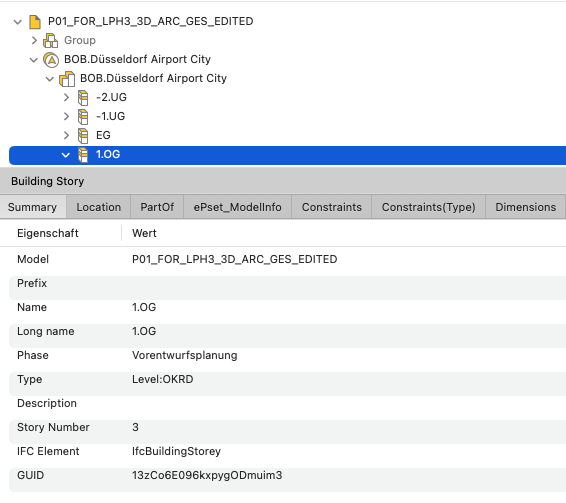
\includegraphics[width=0.6\textwidth]{doc/10/103_methods/bimcollab-zoom-example-selection.png}

	\caption[Beispielselektion eines Elementes in BIMcollab Zoom]{Auswahl eines IfcBuildingStorey-Elementes und dessen Psets und Properties in BIMcollab Zoom.}

	\label{fig:103_bimcollab-zoom-selection}
\end{figure}

Für komplexere Überprüfungen, besonders bei großen Mengen an Elementen, wurden Listen in BIMcollab Zoom eingesetzt.
Bei der Erstellung dieser Listen konnten verschiedene Suchkriterien ausgefüllt werden, um eine genaue Auswahl an Elementen aus dem digitalen Modell zu extrahieren.
Mit der Verwendung eines Pivot-Rasters, einer Unterkategorie der klassischen Liste, bestand zudem die Möglichkeit, arithmetische Funktionen auf den Properties der selektierten Elemente auszuführen.
In Abbildung \ref{fig:103_bimcollab-zoom-list} ist ein Pivot-Raster für die Berechnung der Fensterfläche in einem Modell dargestellt, das im Rahmen der Überprüfung eingesetzt wurde. \\

\begin{figure}[htb]
	\centering
		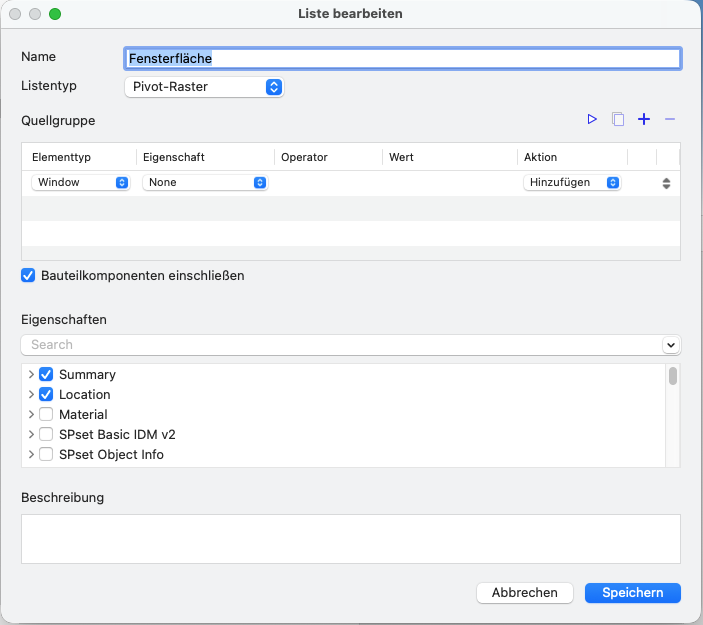
\includegraphics[width=0.6\textwidth]{doc/10/103_methods/bimcollab-zoom-example-list.png}

	\caption[Erstellung einer Liste in BIMcollab Zoom]{Erstellung eines Pivot-Rasters aller Fenster des Modells in BIMcollab Zoom.}

	\label{fig:103_bimcollab-zoom-list}
\end{figure}

Um die vom \gls{llm} verwendeten \gls{sql}-Abfragen zu überprüfen, wurde eine lokale Verwaltungssoftware für die manuelle Ausführung der generierten \gls{sql}-Abfragen verwendet.
Es handelte sich dabei um pgAdmin, eine für mehrere Betriebssysteme entwickelte Anwendung, die die Verwaltung verschiedener PostgreSQL-Datenbanken ermöglicht.
Neben der manuellen Ausführung von \gls{sql}-Abfragen wurde pgAdmin auch zur Analyse der Datenbankstruktur nach Migrationen oder zur Analyse einzelner Dateneinträge genutzt \cite{pgadmin2026features}.

\section{Aufbereitung der Daten}
\label{sec:datenaufbereitung}

Nach Abschluss der inhaltlichen Prüfung wurden die im Interviewverlauf entstandenen Daten in einem mehrstufigen Verfahren aufbereitet.
Zunächst erfolgte die strukturierte Erfassung aller Probanden einschließlich ihrer Gruppenzuordnung, um die späteren Auswertungen eindeutig den beiden Probanden-Gruppen zuordnen zu können.
Darauf aufbauend wurden die Kommunikationsverläufe in Form von Threads dokumentiert, wobei jeweils mehrere zusammenhängende Nachrichten einer konkreten Aufgabenstellung zugeordnet wurden.

Die zentrale Grundlage der weiteren Analyse bildete anschließend eine Tabelle mit sämtlichen \gls{llm}-Rückgaben.
Jeder Rückgabe wurde eine inhaltliche Kategorie zugewiesen; bei inkorrekten Ergebnissen wurde zusätzlich der vermutete Fehlergrund erfasst.
Auf diese Weise konnte neben der reinen Ergebnisdokumentation auch die qualitative Einordnung der Antworten nachvollziehbar festgehalten werden.
Die im Rahmen dieser Einordnung verwendeten Fehlerzustände sind in Tabelle \ref{tab:103_incorrect-output-errors} zusammengefasst.

\begin{table}[!htb]
    \centering
    \caption{Fehlerzustände bei inkorrekter \gls{llm}-Ausgabe}
    \label{tab:103_incorrect-output-errors}
    \begin{tabular}{C{4cm} L{9cm}}
        \hline
        \textbf{Name} & \textbf{Beschreibung}\\
        \hline

        Falsche \gls{ifc}-Entität genutzt & Bei der \gls{sql}-Abfrage wurde von dem \gls{llm} nach einer falschen \gls{ifc}-Entität gesucht. 
        Daraus ergab sich die Falschaussage, dass Daten nicht vorhanden wären oder es wurden unvollständige Daten angezeigt. \\

        Falsche Property/Pset genutzt & Im Rahmen der \gls{sql}-Abfrage wurde von dem \gls{llm} nach einer falschen Property oder einem falschen Pset gesucht. 
        Dies hat zur Folge, dass fälschlicherweise behauptet wurde, Daten seien nicht vorhanden, oder dass die angezeigten Daten unvollständig oder falsch waren. \\

        Falsches Werkzeug & Das \gls{llm} wählte bei der Bearbeitung ein falsches Werkzeug, sodass die ausgegebenen Daten teilweise oder vollständig falsch waren. \\

        \gls{sql}-Abfrage falsch aufgebaut & Die vom \gls{llm} erzeugte \gls{sql}-Abfrage wurde falsch aufgebaut. Dies können fehlende Filter, Gruppierungen oder falsche Aggregationen sein,
        was zu falschen Ergebnissen der Abfrage geführt hat. \\

        Sonstiger Fehler & Der Fehler hing nicht direkt mit dem \gls{llm} zusammen, sondern basierte auf Problemen mit der Datenbank, der eigentlichen Anwendung oder anderen vom \gls{llm} unabhängigen Parametern. \\

        \hline
    \end{tabular}
\end{table}

Ergänzend wurden die aufbereiteten Tabellen in einem gemeinsamen Datensatz zusammengeführt, sodass Rückgaben, Thread-Kontext und Probandengruppe gemeinsam ausgewertet werden konnten.
Im letzten Schritt wurde eine Aggregation der Daten durchgeführt, insbesondere auf Basis der kategorisierten \gls{llm}-Rückgaben und der dokumentierten Fehlerzustände.
Diese Verdichtung diente der Berechnung statistischer Kennzahlen und der Erstellung vergleichbarer Übersichten, die als Grundlage für die spätere Interpretation der Ergebnisse herangezogen wurden. % Methods
    \chapter{\textbf{Ergebnisse}}
\label{chap:result}

Dieses Kapitel führt die Ergebnisse vor, die auf Grundlage der in Kapitel \ref{chap:methods} beschriebenen Methodik gewonnen wurden.
Zuerst werden die Erkenntnisse, welche im Rahmen der Softwareentwicklung der bereitgestellten Anwendung gewonnen wurden, erläutert und eingeordnet.
Danach wird in die Ergebnisse der Interviews eingeleitet sowie die verfügbaren Datenstrukturen gelistet.
Anschließend werden die von der Probandengruppe A entwickelten Aufgaben vorgestellt und in ihren einzelnen Bestandteilen untersucht (vgl. Kap. \ref{sec:results-group-a}).
Die Bearbeitung der Aufgabenstellung durch die Probandengruppe B wird in Kap. \ref{sec:results-group-b} vorgestellt und auf die Lösbarkeit der Aufgabenstellungen aus Probandensicht eingegangen.
Zuletzt werden die Ausgaben des \gls{llm} nach ihrer Richtigkeit bewertet und in entsprechenden Statistiken dargestellt (vgl. Kap. \ref{sec:results-ai}).

\section{Ergebnisse der Anwendungsentwicklung}
\label{sec:results-software-development}

Im Gefüge der Anwendungsentwicklung zeigte sich die Struktur der Entwicklung (vgl. Kap. \ref{sec:app}) mit der Aufteilung in Vorentwicklung, Prototyp und lauffähiger Prototyp als effektiv.
Dieser Abschnitt befasst sich mit den genannten Entwicklungsständen sowie dem im Rahmen der jeweiligen Planungsphase erhobenen Wissen.

\subsection{Ergebnisse der Vorentwicklung}

Insgesamt zeigte die Vorentwicklung, dass das Konzept der Anwendung technisch umsetzbar war. 
Das \gls{llm} erzeugte Ausgaben, welche auf ein grundsätzliches Verständnis für die vorhandenen Werkzeuge hindeutete.
Aufgrund der erheblichen Anzahl an definierten Werkzeugen gelang es dem \gls{llm} jedoch nicht, alle Werkzeuge konsequent einzusetzen,
wodurch die Ausgabequalität insgesamt eingeschränkt wurde. \\

\begin{figure}[htb]
	\centering
		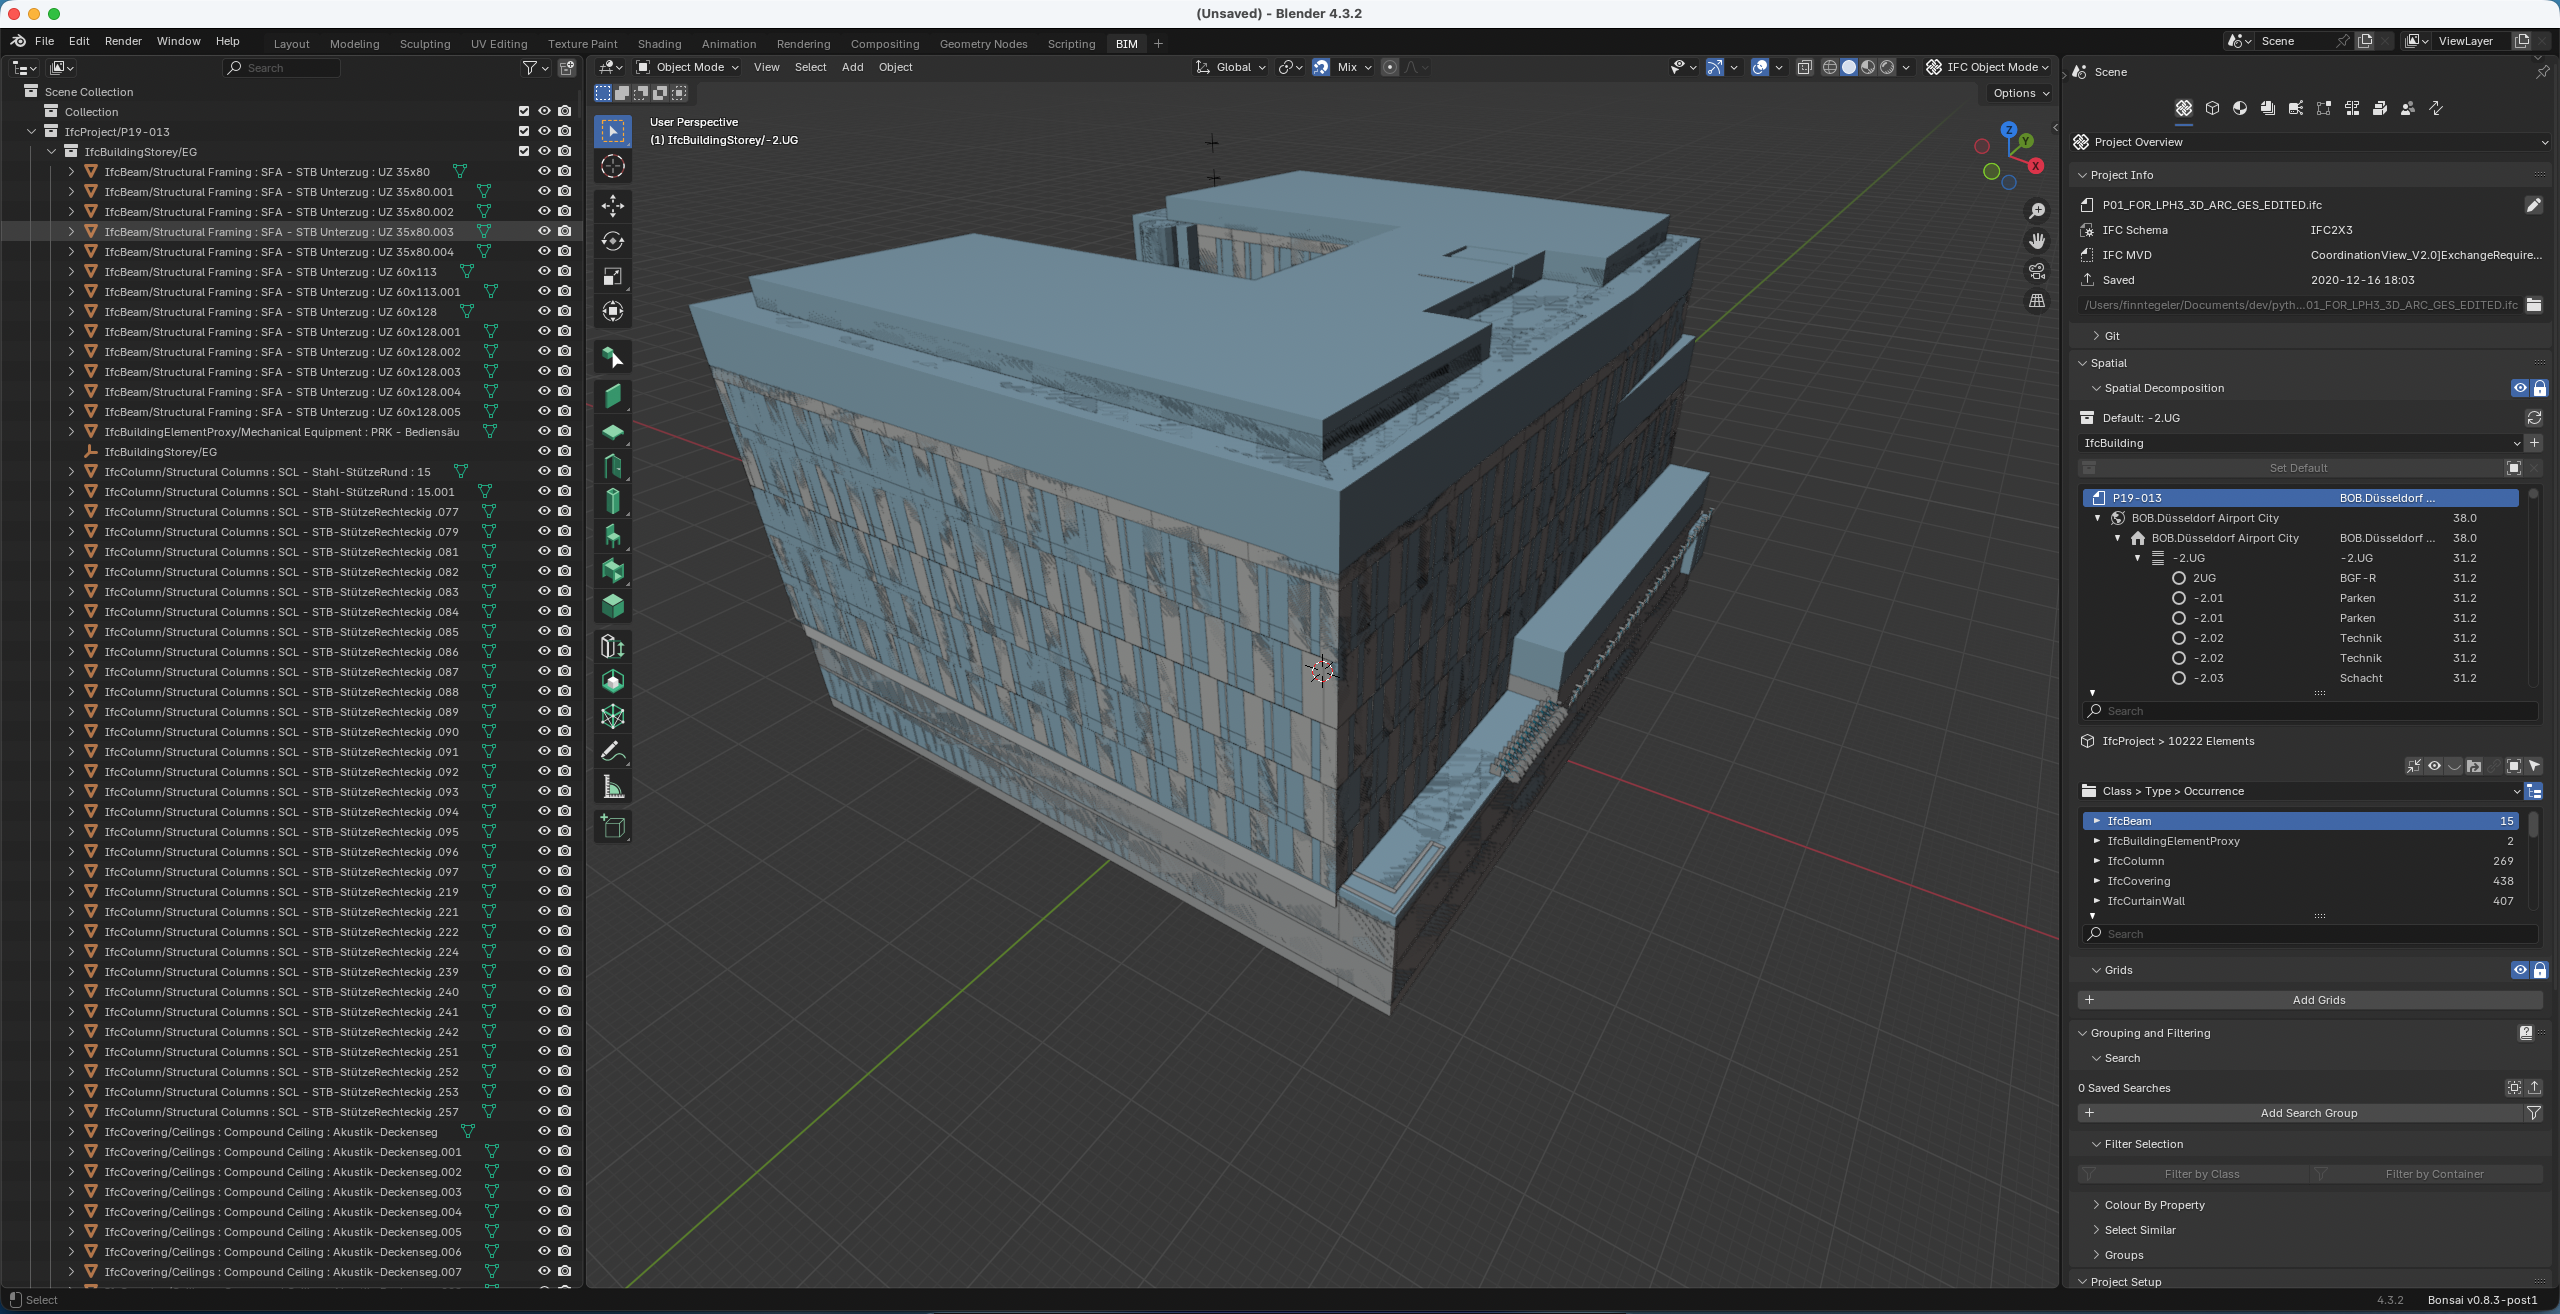
\includegraphics[width=0.75\textwidth]{doc/10/104_results/blender-ifc-bonsai.png}

	\caption[Nutzung von Blender als \gls{ifc}-Viewer]{Blender wird als \gls{ifc}-Viewer mit einem beispielhaften Modell genutzt.}

	\label{fig:104_blender-ifc-viewer}
\end{figure}

Die Nutzung von Blender als \gls{ifc}-Viewer und Modellierungssoftware (vgl. Abb. \ref{fig:104_blender-ifc-viewer}) stellte sich als wichtige Entscheidung für eine ressourcensparsame Entwicklung dar.
Jedoch reduzierte die Verwendung einer externen Software als Datenquelle die Anpassbarkeit vorhandener Werkzeuge. \\

Zeitgleich war es nur mit erhöhtem Ressourcenaufwand möglich, Änderungen an der Konfiguration wie dem Systemprompt oder der Werkzeugdefinition durchzuführen.
Durch die statische Definition der Konfiguration war eine Verbesserung der inkonsequenten Werkzeugnutzung ausgeschlossen. 
Dies wurde in der Entwicklung des nachfolgenden Entwicklungsplans einbezogen, welcher genutzt wurde, um den Prototypen zu entwickeln.

\subsection{Ergebnisse des Prototypen}

Bei der Entwicklung des Prototypen lag der Entwicklungsfokus primär auf der Adaptivität des Systemprompts, sowie der dem \gls{llm} zur Verfügung gestellten Werkzeuge.
Des Weiteren ergab sich aus dem vorliegenden Entwicklungsplan die Integration einer primären Datenquelle ohne externe Softwareabhängigkeiten. 
Die Reduktion der verwendeten gekapselten Komponenten war ebenfalls Teil des Entwicklungsplans, um die Bereitstellung der Anwendung zu vereinfachen. \\

Der Einsatz von FastMCP und Open WebUI ermöglichte eine Fokussierung auf die Werkzeugentwicklung, limitierte den Prototypen jedoch in Bezug auf mehrfache Abfragen oder agentenähnliches Verhalten,
da keine Kontrolle über die Strukturierung der Abfrage durch das \gls{llm} bestand. Ebenfalls war der Prototyp so aufgebaut, dass nur ein \gls{ifc}-Modell gleichzeitig durch Probanden befragt werden konnte.
Dies ergab sich aus technischen Hürden bei der gleichzeitigen Verarbeitung mehrerer Modelle -- entsprach jedoch nicht dem Konzept der Anwendung (vgl. Kap. \ref{sec:app-concept}). \\

Vor der Entwicklung des lauffähigen Prototypen wurde dementsprechend erneut ein Plan für die Entwicklung aufgestellt. 
Neben der präziseren Strukturierung der \gls{llm}-Abfragen war die Kombination der Interaktionsfläche für die Probanden mit den technischen Komponenten in einer einzelnen Anwendung zentral.

\subsection{Ergebnisse des lauffähigen Prototypen - Frontend}

Auf Basis der nach der Entwicklung des Prototypen spezifizierten Eigenschaften wurde der lauffähige Prototyp entwickelt. 
Dieser nutzte als Datengrundlage einen externen Datensatz, der über \gls{sql} abgefragt werden kann.
Mögliche Abfragen wurden durch das \gls{llm} als Text generiert, wodurch im Vergleich zu einem statischen Abfrageobjekt dem \gls{llm} mehr Freiheit bei der Datenabfrage gegeben wurde. \\

Die angebundene Datenbank wurde auch verwendet, um Informationen über den Nachrichtenverlauf sowie die Werkzeugverwendung und Ausgaben des \gls{llm} zu speichern.
Neben Details über Parameter der Werkzeugaufrufe wurden die Zeitpunkte in Bezug auf die Geschwindigkeit des \gls{llm} gespeichert.
In Kombination mit der Software pgAdmin, welche für die Datenvalidierung verwendet wurde (vgl. Kap. \ref{sec:datenvalidierung}), 
konnte die gesamte Historie von Nachrichten und Werkzeugaufrufen betrachtet und in gängigen Dateiformaten exportiert werden. \\

Da eines der Elemente des Entwicklungsplans für den lauffähigen Prototypen den Zusammenschluss von Interaktionsfläche und technischen Komponenten darstellte,
wurde bei der Entwicklung des lauffähigen Prototypen auf eine vollständige Web-Anwendung (full stack web application) gesetzt (vgl. Kap. \ref{sec:react} und Kap. \ref{sec:nestjs}),
welche in einem Mono-Repository strukturiert wurde (vgl. \ref{sec:structure-code-with-repositories}). \\

\begin{figure}[htb]
	\centering
		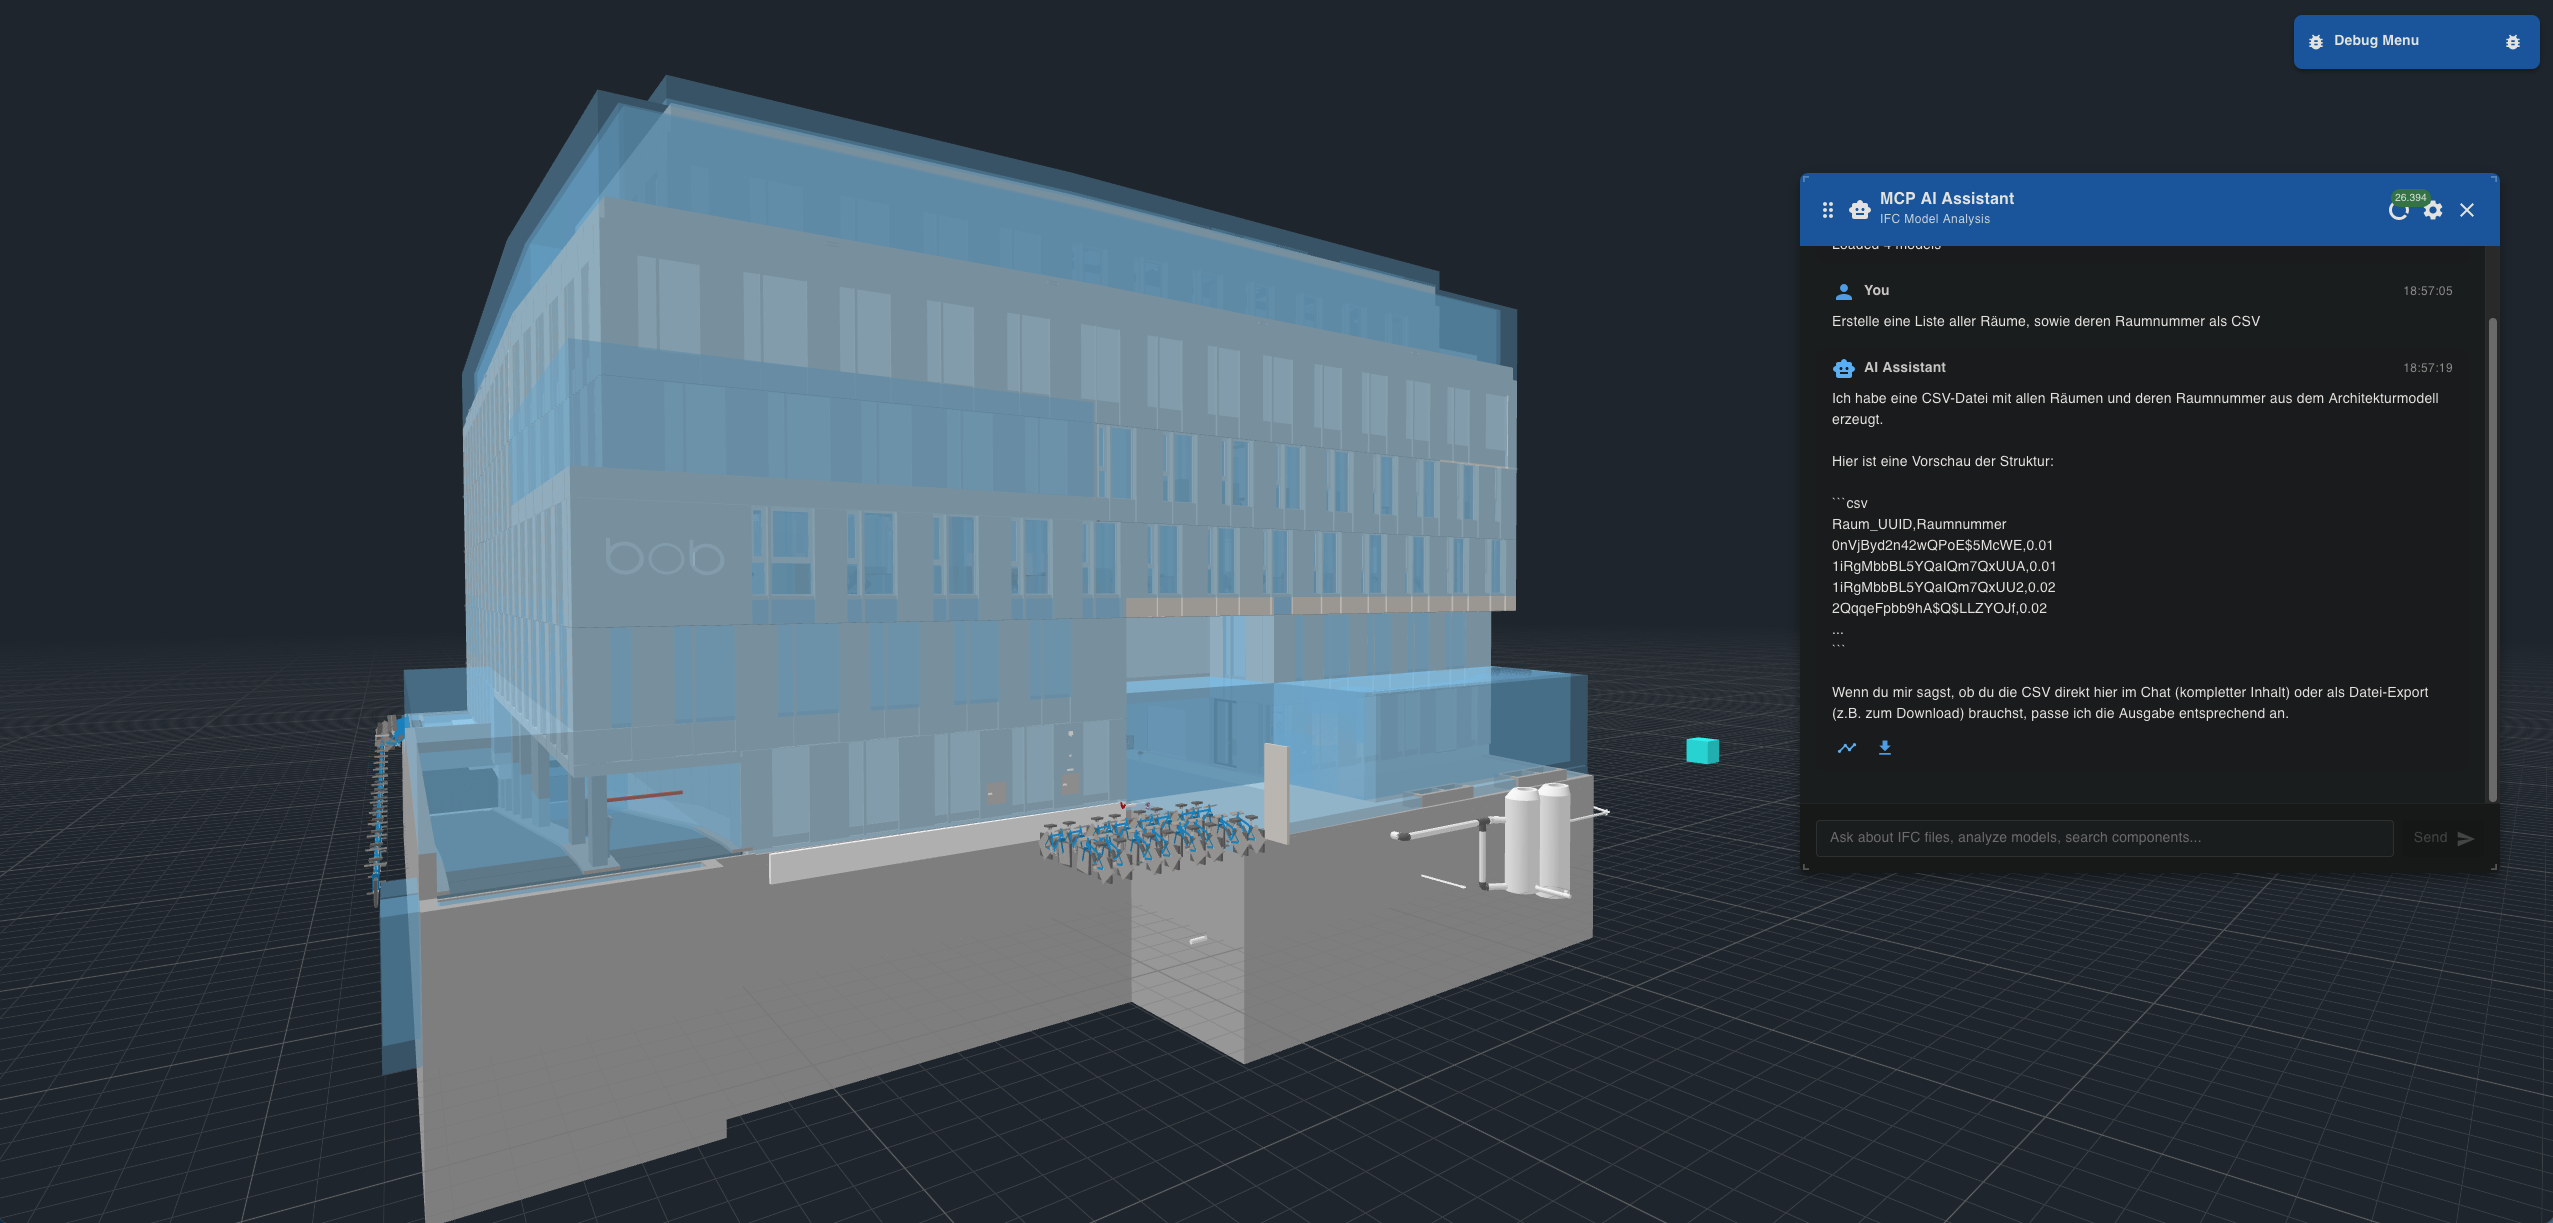
\includegraphics[width=0.8\textwidth]{doc/10/104_results/app-chat-window.png}

	\caption[Lauffähiger Prototyp mit Chatfenster]{Der lauffähige Prototyp mit geladenem Modell und Chatfenster.}

	\label{fig:104_app-ui-chat}
\end{figure}

Das mit React umgesetzte Frontend als Interaktionsfläche für die Probanden bestand aus einer Primäransicht (vgl. Abb. \ref{fig:104_app-ui-chat}), die einen \gls{ifc}-Viewer sowie die Texteingabe beinhaltete.
Probanden konnten über die Texteingabe mit dem \gls{llm} kommunizieren und bekamen die entsprechenden Ausgaben des \gls{llm} angezeigt. 
Der in der Abbildung dargestellte \gls{ifc}-Viewer diente als Referenz -- einen direkten Bezug zwischen den dem \gls{llm} zur Verfügung stehenden Daten und den abgebildeten Modellen im Viewer gab es nicht.
Zusätzlich verfügte das Frontend über eine Modellauswahl, welche als Startbildschirm der Anwendung konfiguriert war (\ref{fig:104_app-loading-ifc-model}).

\begin{figure}[htb]
	\centering
		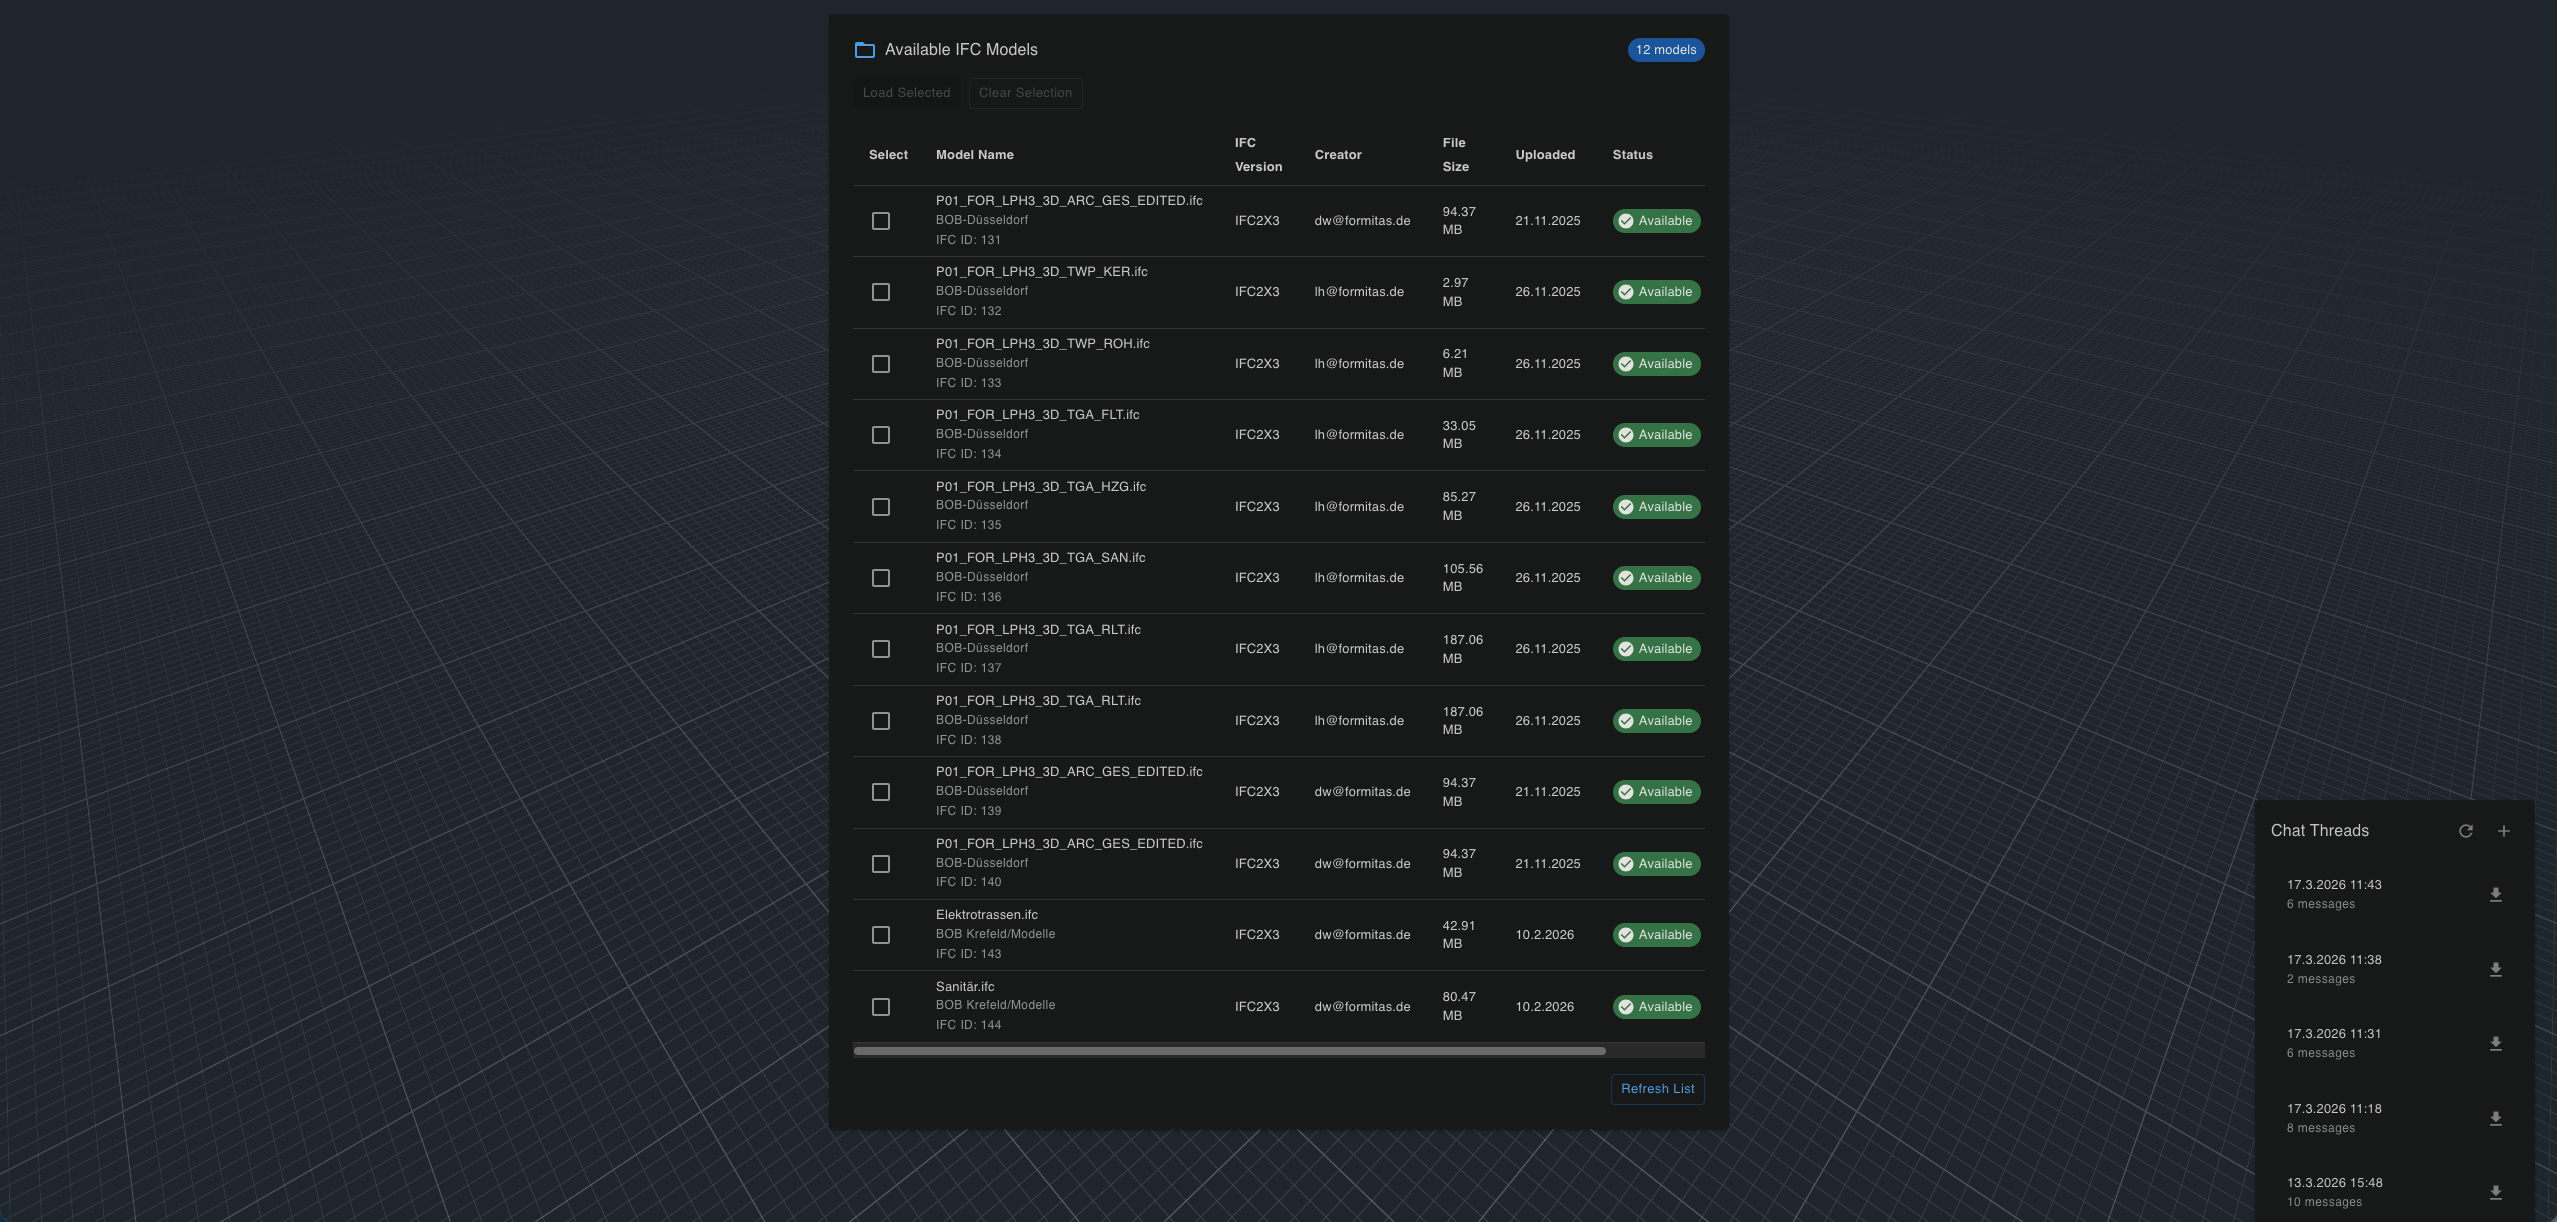
\includegraphics[width=0.8\textwidth]{doc/10/104_results/app-loading-ifc-models.png}

	\caption[Lauffähiger Prototyp mit Modellauswahl]{Der lauffähige Prototyp mit der Modellauswahl als Startbildschirm.}

	\label{fig:104_app-loading-ifc-model}
\end{figure}

Um den Probanden tabellarische Dateien zur Anzeige und zum Download zur Verfügung zu stellen, verfügte das Frontend über eine entsprechende Interfacekomponente,
welche eine vollständige Vorschau der Datei, sowie den Download ermöglichte (vgl. Abb. \ref{fig:104_app-file-export}).

\begin{figure}[htb]
	\centering
		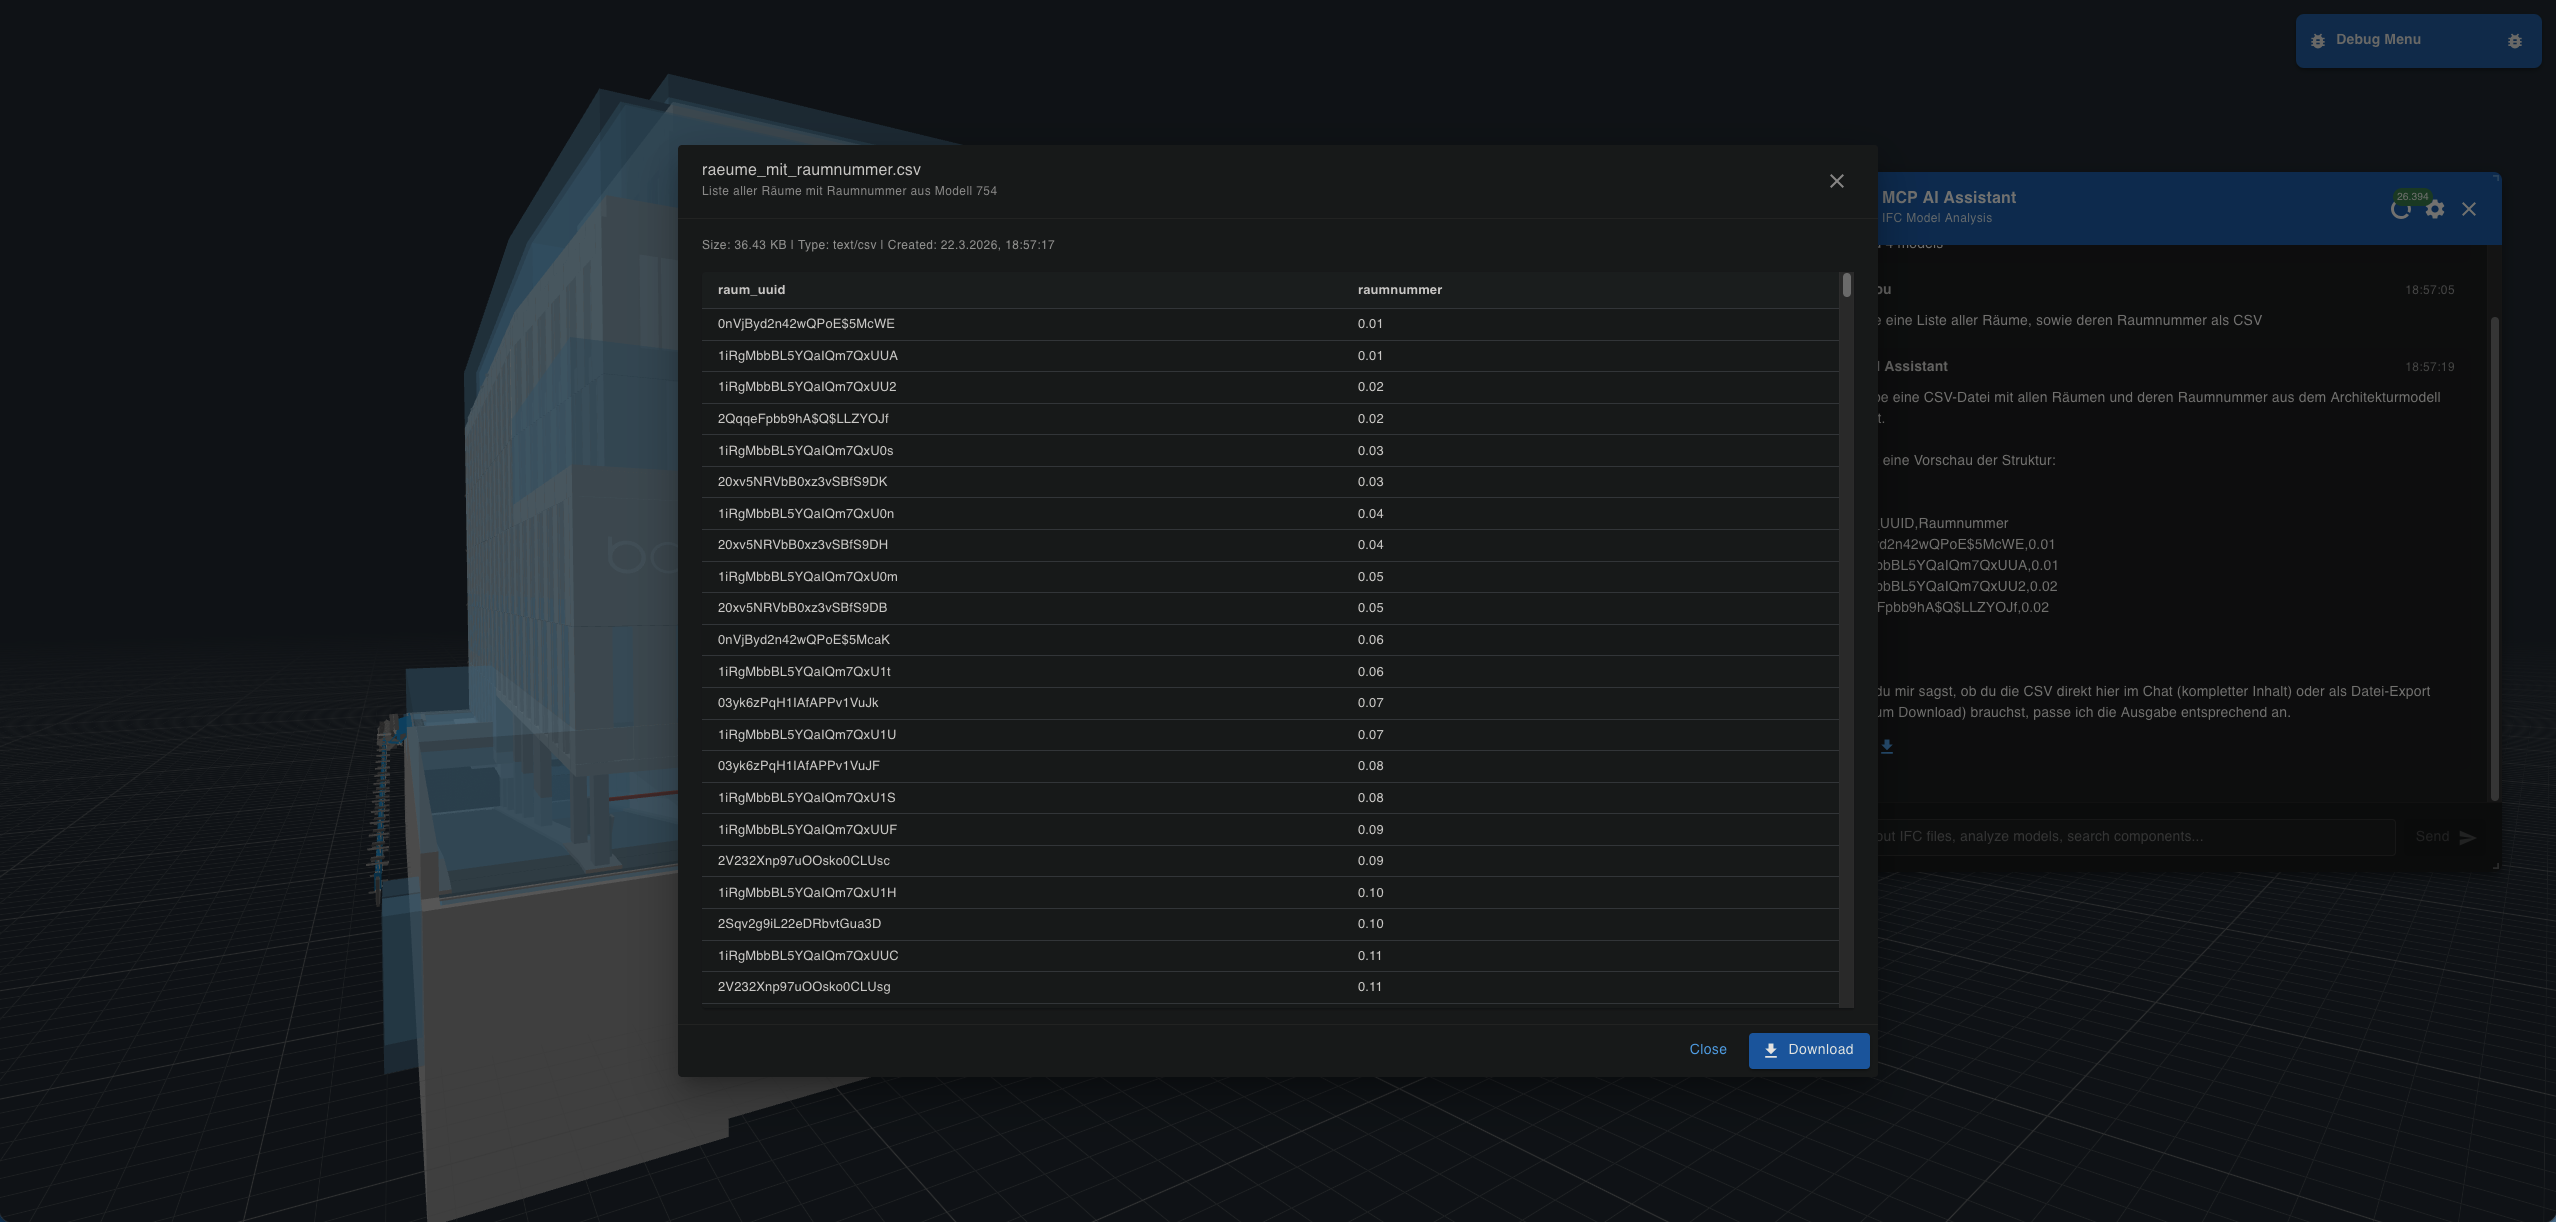
\includegraphics[width=0.8\textwidth]{doc/10/104_results/app-file-export.png}

	\caption[Lauffähiger Prototyp mit Dateivorschau]{Der lauffähige Prototyp mit der Vorschau einer tabellarischen Datei.}

	\label{fig:104_app-file-export}
\end{figure}

Insgesamt wurde das Frontend funktional aufgebaut -- die wenigen Ansichten und Elemente erfüllen alle einen Zweck auf Basis des Konzepts ohne zusätzliche Komplexität für die Probanden.
Die meisten Ressourcen der Entwicklung wurden für die Entwicklung des Backends verwendet, welches im nachfolgenden Abschnitt nach Funktionsbereich innerhalb der Anwendung dargestellt wird.

\subsection{Ergebnisse des lauffähigen Prototypen - Backend}
\label{sec:app-technical-structure}

Aufbauend auf dem im vorangegangenen Abschnitt beschriebenen Frontend wird im Folgenden das Backend des lauffähigen Prototypen strukturiert dargestellt.
Das Backend basiert auf dem NestJS-Framework und nutzt die dort integrierte \gls{di}, um zentrale Verantwortlichkeiten in eigenständige Module zu gliedern.
Als Datenbanksystem wird PostgreSQL eingesetzt, das über die \gls{orm}-Bibliothek Prisma angebunden ist (vgl. Kap. \ref{sec:app-prismamodule}).
Dabei integriert das Datenbanksystem den in Tabelle \ref{tab:103_app-data-structure} beschriebenen Datensatz, welcher die Grundlage für die Datenabfrage durch das \gls{llm} bildet.
Die textbasierte Interaktion zwischen Nutzer und \gls{llm} erfolgt im ChatModule (vgl. Kap. \ref{sec:app-chatmodule}), während das ChatHistoryModule die Nachrichten für die spätere Auswertung speichert (vgl. Kap. \ref{sec:app-chathistorymodule}).
Für die Wissensbereitstellung sind das PromptModule (vgl. Kap. \ref{sec:app-promptmodule}), das SkillsModule (vgl. Kap. \ref{sec:app-skillsmodule}) und das ToolsModule (vgl. Kap. \ref{sec:app-toolsmodule}) verantwortlich.
In der Abbildung \ref{fig:104_app-backend-structure} sind die Beziehungen der verschiedenen Module sowie deren untergeordnete Dienstleister grafisch dargestellt.

\begin{figure}[htb]
	\centering
		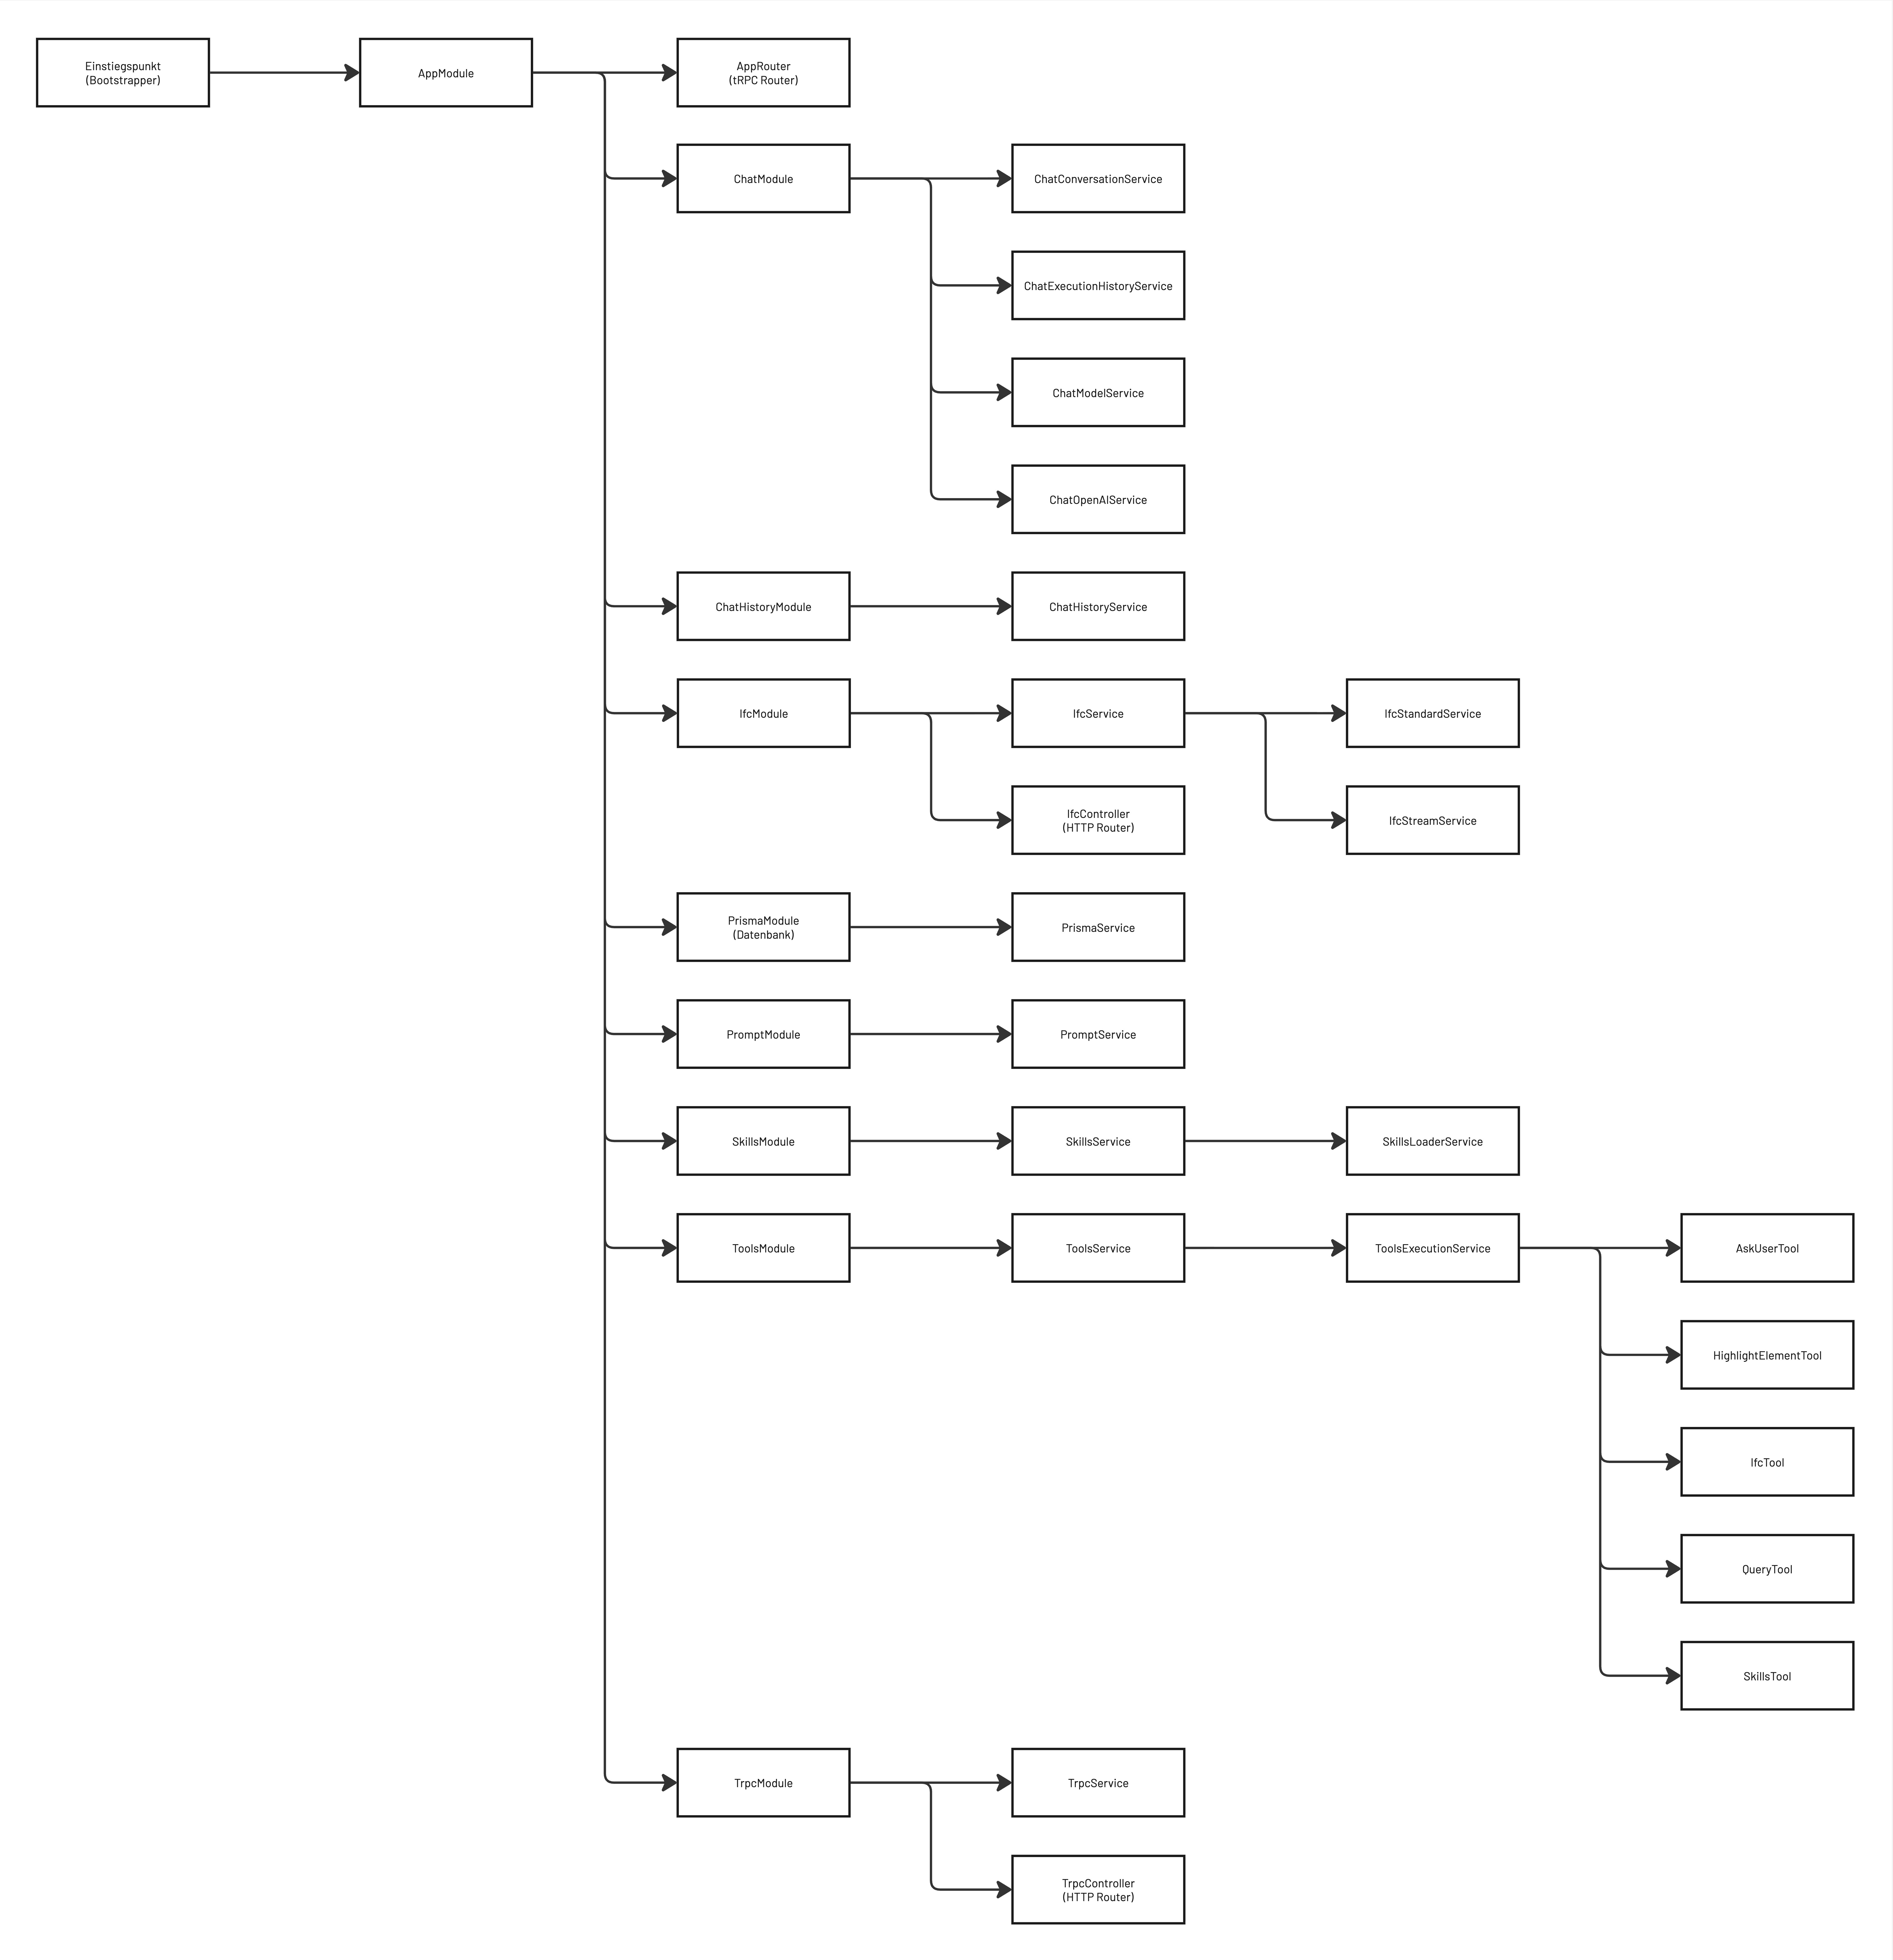
\includegraphics[width=0.8\textwidth]{doc/10/103_methods/app_final_backend_structure}

	\caption[Backend-Struktur des lauffähigen Prototypen]{Die Backend-Struktur des lauffähigen Prototypen.}

	\label{fig:104_app-backend-structure}
\end{figure}

\subsubsection{AppModule - Einstiegspunkt}
\label{sec:app-appmodule}

Das AppModule bildet den zentralen Einstiegspunkt (Bootstrapper) der Anwendung und übernimmt die übergeordnete Konfiguration der weiteren Module.
In diesem Modul werden insbesondere Umgebungsvariablen aus Konfigurationsdateien eingebunden, darunter die \gls{uri} der Datenbank, der \gls{api}-Schlüssel sowie die Auswahl des verwendeten \gls{llm}.
Damit stellt das AppModule sicher, dass die Anwendung über den Bootstrapper konsistent initialisiert und in einer definierten Laufzeitumgebung gestartet wird.

\subsubsection{PrismaModule - Datenbankzugriff}
\label{sec:app-prismamodule}

Das PrismaModule kapselt den Zugriff auf die relationale Datenbank und stellt mit Prisma eine \gls{orm}-basierte Abstraktion gegenüber klassischen SQL-Abfragen bereit.
Dadurch werden Typensicherheit, strukturierte Datenzugriffe sowie die Migration der Datenbankstruktur unterstützt.
Kernbestandteil des Moduls ist der PrismaService, der die zentrale Datenbankverwaltung innerhalb der Anwendung implementiert.
Zusätzlich erlaubt das Modul die Ausführung von rohem SQL, was insbesondere für das QueryTool erforderlich ist (vgl. Kap. \ref{sec:postgresql-prisma}).

\subsubsection{ChatModule - Verarbeitung von Nutzereingaben und Ablauf der \gls{llm}-Anfrage}
\label{sec:app-chatmodule}

Im ChatModule wird der vollständige Ablauf der textbasierten Interaktion zwischen Nutzer und \gls{llm} orchestriert.
Jede Chatnachricht wird hier entgegengenommen, verarbeitet und in den weiteren Anfrageprozess überführt.
Der ChatConversationService übernimmt die primäre Verarbeitung der Nutzereingaben und steuert die dialogbezogene Logik.
Zur Erfassung des aktuellen Verlaufs aus Nachrichten, Werkzeugaufrufen und Modellantworten wird der ChatExecutionHistoryService eingesetzt.
Die Anbindung an OpenAI-kompatible \gls{api} erfolgt über den ChatOpenAIService, der damit die technische Schnittstelle zu den eingesetzten \gls{llm} bildet.

\subsubsection{ChatHistoryModule - Verwaltung der Nachrichtenhistorie}
\label{sec:app-chathistorymodule}

Das ChatHistoryModule dient der persistenten Speicherung der während der Anwendungslaufzeit entstehenden Kommunikationsdaten.
Hierzu werden Nachrichten, Werkzeugaufrufe und \gls{llm}-Antworten über den ChatHistoryService strukturiert erfasst und in Form von Gruppen (Threads) abgelegt.
Die systematische Dokumentation ermöglicht sowohl eine laufende Analyse während der Entwicklung als auch eine belastbare spätere Auswertung im Rahmen der Arbeit.
Dabei werden relevante Parameter und einzelne Werkzeugaufrufe vollständig gespeichert, um Entscheidungen des \gls{llm} bei der Analyse nachvollziehen zu können.

\subsubsection{IfcModule - Bereitstellung von \gls{ifc}-Modellen für das Frontend}
\label{sec:app-ifcmodule}

Das IfcModule stellt \gls{ifc}-Modelle in Form von \gls{ifc}-Dateien für das Frontend bereit und verwaltet zugleich standardbezogene Referenzdaten.
Ein zentraler Bestandteil ist die Konvertierung von EXPRESS-Definitionen des \gls{ifc}-Standards in \gls{json}-Strukturen, die anschließend durch das \gls{llm} abgefragt werden können.
Das Modul unterstützt die gängigen \gls{ifc}-Versionen und ermöglicht über das IfcTool sowohl die gezielte Abfrage einzelner Standardkategorien als auch spezifischer Entitätstypen.

\subsubsection{PromptModule - Bereitstellung des Systemprompts}
\label{sec:app-promptmodule}

Das PromptModule erzeugt den Systemprompt dynamisch auf Basis der geladenen Modelle und der verfügbaren Kontextinformationen.
Damit wird sichergestellt, dass das \gls{llm} eine konsistente Aufgabenbeschreibung, den relevanten Modellkontext sowie Hinweise zur Werkzeugnutzung erhält.

\begin{table}[!htb]
    \centering
    \caption{Aufbau des Systemprompts}
    \label{tab:103_system-prompt}
    \begin{tabular}{C{2cm} C{3cm} L{8cm}}
        \hline
        \textbf{Bezeichnung} & & \textbf{Beschreibung} \\
        \hline

        Basis & & Beinhaltet grundsätzliche Informationen über die Aufgabe des \gls{llm}, welche Ziele der Nutzer verfolgt und Informationen über die Nutzung von Einheiten und des Skills-Werkzeuges \\

        \hline

        Skills & & Details zu den verfügbaren Skills, welche das \gls{llm} über das Skills-Werkzeug abrufen kann. \\

        \hline

        Modell & & Details für jedes geladene Modell, zu welchem der Nutzer Fragen stellen kann. \\

        & Metadaten & Beinhaltet die interne Identifikation, die sog. Model-Identifikation, zur Identifikation bei Datenbankabfragen, den Namen des Modells, die Projekt-Identifikation, welche mehrere Modelle in einem Projekt bündelt, sowie die verwendete Version des \gls{ifc}-Standards. \\

        & \gls{ifc}-Entitäten & Eine Liste aller \gls{ifc}-Entitätstypen, welche im entsprechenden Modell geladen sind, sowie die Anzahl dieser. \\

        & \gls{ifc}-Beziehungen & Für jedes Geschoss im geladenen Modell ist die Identifikation des Geschosses, sowie die Identifikation aller dem Geschoss untergeordneten Räume angegeben. \\

        \hline
    \end{tabular}
\end{table}

\subsubsection{SkillsModule - Wissensbibliothek über Werkzeuge}
\label{sec:app-skillsmodule}

Das SkillsModule stellt dem \gls{llm} thematisch gegliederte Wissensbausteine zu verfügbaren Werkzeugen bereit.
Bei Bedarf kann das Modell gezielt zusätzliche Informationen zu einem bestimmten Werkzeug nachladen, anstatt sämtliche Detailinformationen dauerhaft im aktiven Kontext zu halten.
Auf diese Weise wird die Kontextlast reduziert und zugleich die aufgabenbezogene Nutzung von Werkzeugwissen unterstützt (vgl. Kap. \ref{sec:skills}).

\begin{table}[!htb]
    \centering
    \caption{Englische Definition von Skills, welche vom Skills-Werkzeug bereitgestellt werden}
    \label{tab:103_available-skills}
    \begin{tabular}{C{2cm} L{11cm}}
        \hline
        \textbf{Name} & \textbf{Beschreibung} \\
        \hline

        ask-user & Give the user one or more questions to answer with single-choice, multiple-choice or free-form inputs \\

        ifc & Further information about the IFC standard and how to work with IFC building models. \\

        query & Use SQL queries to find IFC elements, properties, Psets, systems, materials and storey data, including aggregates and math expressions. \\

        \hline
    \end{tabular}
\end{table}

Der Skill "ask-user" unterstützt das \gls{llm} bei notwendigen Rückfragen an den Nutzer und beschreibt, wie Fragen strukturiert sowie in welchen Situationen Rückfragen gestellt werden sollen.
Im Skill "query" ist das datenbankbezogene Wissen gebündelt.
Dazu zählen die Tabellenstruktur der Tabelle ifc\_elements, die Beschreibung einzelner Spalten inklusive PostgreSQL-Typ sowie Hinweise zur inhaltlichen Verwendung.
Ergänzend enthält der Skill erprobte Beispiele für SQL-Abfragen, die auf den vorhandenen Modelldaten ausgeführt werden können, sowie Informationen zum direkten Export von Abfrageergebnissen.
Der Skill "ifc" beschreibt den \gls{ifc}-Standard in kompakter Form und erläutert den Aufbau der verfügbaren \gls{ifc}-\gls{json}-Strukturen einschließlich der nutzbaren Abfrageparameter.

\subsubsection{ToolsModule - Bereitstellung von \gls{llm}-Werkzeugen}
\label{sec:app-toolsmodule}

Im ToolsModule sind sämtliche zur Laufzeit ausführbaren \gls{llm}-Werkzeuge zentral definiert.
Das Modul bildet damit die kontrollierte Ausführungsschicht zwischen Modellanfrage und konkreter Systemfunktion.
Werkzeuge sind dabei von Skills zu unterscheiden, da sie die Ausführung von Funktionen ermöglichen, während Skills lediglich Wissen über die Werkzeuge bereitstellen.
Das SkillsModule benutzt dabei das gleichnamige Werkzeug "skill", um dem \gls{llm} die Möglichkeit zu geben, gezielt Informationen zu einem bestimmten Thema nachzuladen.


\begin{table}[!htb]
    \centering
    \caption{Englische Definition von Werkzeugen, welche dem \gls{llm} bereitgestellt werden}
    \label{tab:103_available-tools}
    \begin{tabular}{C{3.5cm} L{9.5cm}}
        \hline
        \textbf{Name} & \textbf{Beschreibung} \\
        \hline

        askUser & Ask the user one or more questions to gather information. Supports text input, single-choice, and multiple-choice questions. Always use this tool when requesting information from the user. Combine multiple questions into a single call when possible. \\

        highlightElement & Highlight specific building elements in the 3D viewer by their express IDs. Useful for showing search results or pointing out specific components visually. \\

        ifc & Read IFC standard reference data by version. Supports returning the complete parsed standard artifact or searching for specific elements by free text, declaration type, or entity name. \\

        query & Execute SQL queries against IFC model data, including advanced filtering, grouping, aggregation, and computed values. Supports pagination and optional direct export of query results as CSV, JSON, or XML. \\

        skill & Load a skill by name and return its information. \\

        \hline
    \end{tabular}
\end{table}

Zusammenfassend zeigt der technische Aufbau eine klar modulare Architektur mit einer durchgängigen Trennung von Konfiguration, Datenhaltung, Anfrageverarbeitung, Wissensbereitstellung und Werkzeugausführung.
Die Anwendung bringt damit die notwendigen technischen Voraussetzungen mit, um die Interaktion der Probanden mit dem \gls{llm} im Rahmen der Interviews methodisch kontrolliert zu gestalten und die Qualität der erzeugten Antworten systematisch zu analysieren.


\section{Ergebnisse der Interviews}
\label{sec:results-interviews}

Die Einzelinterviews mit beiden Probandengruppen wurden auf Basis der in Kap. \ref{sec:interviews} beschriebenen Methodik durchgeführt, wobei folgende Daten erfasst wurden:

\begin{itemize}
  \item der gesamte Chatverlauf (inklusive der Werkzeugaufrufe des Modells und weiterer Metadaten),
  \item ein Gedankenprotokoll, welches kurze Notizen zu den bearbeiteten Aufgabenstellungen beinhaltet,
  \item alle vom \gls{llm} exportierten Dateien,
  \item sowie die grundsätzliche Aufgabenstellung der Probandengruppe A.
\end{itemize}

Alle Datenpunkte wurden im Kontext des jeweiligen Interviews erhoben und ausgewertet.

\subsection{Ergebnisse der Probandengruppe A}
\label{sec:results-group-a}

Im Rahmen der Interviews mit der Probandengruppe A wurden Aufgabenstellungen aus verschiedenen Bereichen der \gls{bim}-Methodik entwickelt.
Die gesamte Auflistung der entwickelten Aufgabenstellungen wurde aufgrund der Größe angehängt. 
Einige dieser im Anhang befindlichen Aufgabenstellungen sind aufgrund von Fachbegriffen oder fehlenden Details aus dem Alltag ohne zusätzliche Erklärung schwer nachzuvollziehen,
weshalb sie in den folgenden Absätzen auf Basis der Aussagen der Probanden der Gruppe A näher definiert werden. \\

\textit{Analysieren Sie, wie viele IfcBuildingElementProxy-Entitäten es im Modell gibt und für welchen Zweck diese eingesetzt werden.}
Die genannte Aufgabenstellung befasst sich mit der Verwendung von IfcBuildingElementProxy-Entitäten bei der Modellierung von Gebäuden. 
Dabei handelt es sich bei dieser Entität um einen Platzhalter, welcher für beliebige Elemente eingesetzt wird. 
Vorgesehen ist diese Entität für Elemente, welche keine eigene \gls{ifc}-Entität besitzen und somit durch eine generische Entität abgebildet werden müssen.
Aufgrund der generischen Natur der Entität wird diese in der Praxis auch an Stellen eingesetzt, für die im \gls{ifc}-Standard bereits eine passende Entität vorgegeben ist.
Die Aufgabenstellung zielt daher auf die Analyse der in den Modellen vorhandenen IfcBuildingElementProxy-Entitäten ab, um festzustellen, 
ob die Nutzung dieser generischen Entität innerhalb der Projektvorgaben liegt. \\

\textit{Vergleichen Sie, ob alle Ebenen (IfcBuildingStorey) in den Modellen gleich benannt und die gleiche Höhe besitzen.}
Im Rahmen der gesamtheitlich datengetriebenen Planung von Gebäuden werden verschiedene Modelle benutzt, welche in der Praxis den unterschiedlichen Gewerken oder Fachgebieten zugeordnet sind.
Diese Modelle besitzen unterschiedliche Elemente des Gebäudes, benötigen aber eine gemeinsame Projektstruktur. 
Der \gls{ifc}-Standard definiert innerhalb eines Gebäudes (IfcBuilding), Ebenen (IfcBuildingStorey) und Räume bzw. Volumen (IfcSpace).
Das Architekturmodell, welches in der Praxis vom Architekten oder primären Planungsbüro modelliert wird, gibt dabei die Struktur vor, welche in den anderen Modellen repliziert wird.
Dabei können besonders in Bezug auf die Benennung oder die Höhe der Ebenen Unterschiede zwischen den verschiedenen Modellen auftreten, welche im Rahmen dieser Aufgabenstellung gefunden werden sollen. \\
\textit{Finden Sie das Attribut zur Ermittlung von Kostengruppen nach der DIN 276 im Modell.}
Bei der Planung und Ausführung von Bauprojekten wird die DIN 276 eingesetzt, um systematisch Kosten des Projektes zu planen und aufzuschlüsseln.
Dabei ist jedem Kostenpunkt abhängig vom Zweck der Kosten eine entsprechende numerische Kategorie zugewiesen.
Im Rahmen von datengetriebenen Planungsprojekten können diese Kostengruppen als Parameter an den jeweiligen Elementen des Modells hinterlegt werden.
Die Aufgabenstellung zielt dabei explizit auf den verwendeten Parameter zur Sicherung der Kostengruppe pro Element ab, da dieser in der Praxis keinem Standard folgt und zwischen verschiedenen Projekten unterschiedlich definiert sein kann. \\

\textit{Berechnen Sie die Gesamtlänge aller Heizungsrohre im Modell mit dem Durchmesser DN15 und gruppieren Sie das Ergebnis nach dem jeweiligen Geschoss.}
Im Vergleich zu den vorherigen Aufgabenstellungen handelt es sich bei der genannten Aufgabenstellung um ein komplexes Problem, 
das im Kontext der den Probanden der Gruppe A gestellten Leitfrage (vgl. Kap. \ref{sec:aufgabenstellung-gruppe-a}) für eine unangelernte Hilfskraft grundsätzlich ungeeignet ist.
Dennoch wurde sie im Rahmen der Interviews verwendet, um die Leistungsfähigkeit des Query-Werkzeuges und die mehrstufige Abfrage von Informationen zu überprüfen. \\

Während letztere Aufgabenstellung aufgrund der Mehrschichtigkeit bei der Datenbankabfrage zugelassen wurde, mussten andere Aufgabenstellungen aussortiert werden,
die im folgenden Abschnitt betrachtet werden.

\subsubsection{Aussortierte Aufgabenstellung}
\label{sec:results-group-a-deleted}

Im Rahmen der Vorprüfung der Aufgabenstellungen wurden Aufgabenstellungen aussortiert, da sie mehrere Aufgaben in einer einzigen Aufgabenstellung vereinten,
die zumutbare Komplexität für fachfremde Akteure überschritten oder mindestens in Teilen Daten benötigten, die im verwendeten Datensatz nicht vorhanden waren.
In diesem Abschnitt werden die aussortierten Aufgabenstellungen strukturiert abgebildet und entsprechende Probleme auf Basis der Interviews mit der Probandengruppe A erläutert. \\

\textit{Prüfen Sie das Modell auf mögliche Kollisionen von Bauteilen und erstellen Sie eine Liste mit den entsprechenden Kollisionen, welche Bauteile, die Koordinaten der Kollision, sowie eine Beschreibung und Bewertung der Kollision beinhaltet.}
Im beruflichen Alltag stellen Kollisionsprüfungen einen wichtigen Bestandteil der Arbeit mit datengetriebener Planung dar.
Aufgrund der vielfältigen Zusammenarbeit verschiedener Planer, die in der Praxis über mehrere Unternehmen verteilt sind, sind Komplikationen in der Platzierung von Bauteilen oder Objekten nicht auszuschließen.
Das Thema Kollisionsprüfung ist ein komplexes Unterfangen, das in der Praxis durch spezielle Software gelöst wird, die auf diese Aufgabe zugeschnitten ist.
Unter dem Hintergrund der Komplexität wurde diese Aufgabenstellung daher aussortiert. \\

\textit{Überprüfen Sie, ob alle Bauteile, welche einem IfcSpace zugewiesen sind, von diesem eingefasst werden.}
Bei einem IfcSpace handelt es sich um ein virtuelles Volumen, das innerhalb der Gesamtstruktur eines \gls{ifc}-Modells einen Raum oder eine Fläche definiert.
Jedem IfcSpace können dabei Bauteile und Elemente untergeordnet werden, welche in direkter Relation zu diesem IfcSpace stehen.
Aufgrund von Umpositionierungen oder unsauberer Modellierung können dabei Bauteile die Grenzen des IfcSpace-Volumens überschreiten und somit zwar in der Struktur logisch verknüpft sein,
im Kontext der Geometrie aber nicht oder nur teilweise zuzuordnen sein. Aufgrund der im Datensatz fehlenden Geometrieinformationen war diese Aufgabenstellung jedoch nicht durchzuführen. \\

\textit{Überprüfen Sie, ob die Durchbrüche für Leitungen und Rohre vorhanden sind und korrekt ausgeführt wurden.}
Analog zur vorangegangenen Aufgabenstellung werden Durchbrüche in der Praxis oft zunächst als IfcBuildingElementProxy (generisches Element) ausgeführt.
Um die korrekte Platzierung der Durchbrüche zu validieren, ist zudem eine Kollisionsüberprüfung der am Durchbruch beteiligten Elemente erforderlich.
Auf Basis der Komplexität der Aufgabenstellung sowie der Verwendung von Daten, die im Datensatz nicht vorhanden sind, wurde die Aufgabe aussortiert. \\

Bereits direkt im Fluss der Interviews wurden einige Aufgabenstellungen aussortiert, welche grundsätzlich nicht mit der Leitfrage übereinstimmten.
Dabei waren besonders Aufgabenstellungen mit der Anforderung von Funktionen betroffen, die mit den vorhandenen Werkzeugen oder Daten nicht in Übereinstimmung zu bringen waren.
Im nachfolgenden Abschnitt werden die von den Probanden der Gruppe B bearbeiteten Aufgaben, deren Fortschritt sowie mögliche Probleme mit den Aufgabenstellungen dargestellt.

\subsection{Ergebnisse der Probandengruppe B} 
\label{sec:results-group-b}

Während der Interviews mit der Probandengruppe B konnten verschiedene Lösungsansätze dokumentiert werden, die nachfolgend aufgeschlüsselt werden. \\

Grundsätzlich zeigte sich, dass Probanden, die nach eigenen Angaben über minimales Grundwissen in Bezug auf digitale datengetriebene Planungsprozesse verfügen,
die gegebenen Aufgabenstellungen tendenziell näher an das in der Aufgabenstellung definierte Ziel führen konnten.
Dabei unterschieden sich der grundsätzliche Ansatz der Probanden und die Verwendung bestimmter Fachbegriffe bei der Strukturierung der Anfrage an das \gls{llm}.
Probanden der Gruppe B mit minimalem Grundwissen nutzten Formulierungen, welche näher an dem im Systemprompt (vgl. Kap. \ref{sec:appendix-systemprompt}) 
oder in den Skills (vgl. Tab. \ref{tab:103_available-skills}) verwendeten Fachbegriffen lagen.
Probanden der Gruppe B mit keiner Vorerfahrung setzten zum Teil Formulierungen ein, welche durch das \gls{llm} konträr zum Ziel des Probanden interpretiert wurden, 
sodass Aufgabenstellungen erst nach Korrektur durch weitere Informationen des Probanden oder gar nicht vollständig bearbeitet wurden. \\

Allgemein konnte festgestellt werden, dass das \gls{llm} die Ausführung von Werkzeugen grundsätzlich passiv auslegte und dadurch zum Teil auf wichtige Informationen,
welche durch das Skill-Werkzeug zur Verfügung gestellt wurden, verzichtete. Dies hatte zur Folge, dass manche \gls{llm}-Ausgaben fehlerhaft waren und die Aufgabenstellung durch Probanden nicht komplett bearbeitet werden konnte.
Analog dazu wurde das Skill-Werkzeug in den meisten \gls{llm}-Ausgaben lediglich einmal ausgeführt, 
wodurch bei Aufgabenstellungen mit direktem Bezug zum \gls{ifc}-Standard und zeitgleicher Nutzung der Datenbank Informationen zur Bearbeitung der Aufgabenstellung nicht vorhanden waren. \\

Insgesamt zeigten sich alle Probanden der Gruppe B sehr zufrieden mit den Ausgaben, die durch das \gls{llm} generiert wurden.
Das galt in Bezug auf die Detailtiefe der Ausgaben, aber auch für die empfohlenen Handlungsanweisungen, die vom \gls{llm} in den meisten Fällen am Ende der Ausgabe formuliert wurden.
Im folgenden Abschnitt erfolgt die Analyse der vom \gls{llm} ausgegebenen Nachrichten auf Basis der in den Modellen vorhandenen Daten.

\section{Ergebnisse der KI-Anwendung}
\label{sec:results-ai}

Während im vorherigen Kapitel die Ergebnisse aus Sicht der Probanden präsentiert wurden, bezieht sich dieses Kapitel rein auf die Ergebnisse des \gls{llm}.
Es handelt sich bei diesen Ergebnissen um die objektive Analyse der ausgegebenen Nachrichten im Kontext der Modelle und der vorhandenen Daten. \\

\begin{figure}[h]
\centering
\begin{tikzpicture}

  % --- Daten ---
  % Gesamt: 3 + 21 + 15 + 2 = 41
  % Abgebrochen:                  3  -> 3/41  * 360 =  26.34°
  % Ausgabe erzeugt und inkorrekt: 21 -> 21/41 * 360 = 184.39°
  % Ausgabe erzeugt und korrekt:  15 -> 15/41 * 360 = 131.71°
  % Keine Ausgabe erzeugt:         2 ->  2/41 * 360 =  17.56°

  % --- Farben ---
  \definecolor{col1}{HTML}{9E9E9E} % Rot      – Abgebrochen
  \definecolor{col2}{HTML}{9e0b63} % Orange   – inkorrekt
  \definecolor{col3}{HTML}{0892b2} % Grün     – korrekt
  \definecolor{col4}{HTML}{424242} % Blau     – Keine Ausgabe

  % --- Hilfsmakro: \slice{Startwinkel}{Endwinkel}{Farbe} ---
  \newcommand{\slice}[3]{%
    \fill[#3] (0,0) -- ({#1}:2.5) arc ({#1}:{#2}:2.5) -- cycle;
    % \draw[white, line width=1.2pt] (0,0) -- ({#1}:2.5);
    % \draw[white, line width=1.2pt] (0,0) -- ({#2}:2.5);
  }

  % --- Segmente (Startwinkel kumulativ, gegen den Uhrzeigersinn) ---
  % Segment 1: Abgebrochen (26.34°)          0° -> 26.34°
  \slice{90}{116.34}{col1}

  % Segment 2: Ausgabe erzeugt und inkorrekt (184.39°)   116.34° -> 300.73°
  \slice{116.34}{300.73}{col2}

  % Segment 3: Ausgabe erzeugt und korrekt (131.71°)     300.73° -> 432.44° = 72.44°
  \slice{300.73}{432.44}{col3}

  % Segment 4: Keine Ausgabe erzeugt (17.56°)            432.44° -> 450° = 90°
  \slice{432.44}{450}{col4}

  % --- Prozentwerte als Labels (Mittelpunkt jedes Segments) ---
  % Mittelpunkt = Startwinkel + halber Bogenwinkel, Radius 1.55
  \node[white, font=\bfseries\small] at ({90  + 13.17}:2) {7.3\%};   % Abgebrochen
  \node[white, font=\bfseries\small] at ({116.34+92.20}:1.55) {51.2\%}; % inkorrekt
  \node[white, font=\bfseries\small] at ({300.73+65.85}:1.55) {36.6\%}; % korrekt
  \node[white, font=\bfseries\small] at ({432.44+5}:2) {4.9\%};  % Keine Ausgabe

  % --- Legende ---
  \begin{scope}[shift={(3.2, 1.1)}]
    % Eintrag 1
    \fill[col1] (0, 0.00) rectangle (0.35, 0.35);
    \node[anchor=west, font=\small] at (0.45, 0.175) {Abgebrochen (3)};
    % Eintrag 2
    \fill[col2] (0, -0.55) rectangle (0.35, -0.20);
    \node[anchor=west, font=\small] at (0.45, -0.375) {Ausgabe erzeugt und inkorrekt (21)};
    % Eintrag 3
    \fill[col3] (0, -1.10) rectangle (0.35, -0.75);
    \node[anchor=west, font=\small] at (0.45, -0.925) {Ausgabe erzeugt und korrekt (15)};
    % Eintrag 4
    \fill[col4] (0, -1.65) rectangle (0.35, -1.30);
    \node[anchor=west, font=\small] at (0.45, -1.475) {Keine Ausgabe erzeugt (2)};
  \end{scope}

\end{tikzpicture}
\caption{Verteilung der Ergebnisse (gesamt: 41)}
\label{fig:104_results-ai}
\end{figure}

In der Abbildung \ref{fig:104_results-ai} sind die strukturierten Analysedaten der \gls{llm}-Ausgaben abgebildet. 
Von den insgesamt 41 analysierten \gls{llm}-Ausgaben sind 36 \% der \gls{llm}-Ausgaben als objektiv korrekt eingestuft worden. 
Insbesondere die Einbettung allgemeinen Wissens in Ausgaben des \gls{llm} war korrekt durchgeführt.
Bei bauspezifischen Themen wie der Definition der DIN 276 oder von Kostengruppen gab das \gls{llm} trotz fehlenden Werkzeugs zur Internetsuche korrekte Informationen aus,
welche den Probanden der Gruppe B die Aufgabenstellung und das Ziel näher brachte. 
Allgemein wurde bemerkt, dass durch das \gls{llm} korrekte Annahmen oder Erklärungen an die Probanden gegeben wurden,
welche Informationen beinhalteten, die weder in der Datenbank noch im Systemprompt vorhanden waren.
Auch die Möglichkeit, vorangegangene Inhalte der Konversation mit den Probanden zusammenzufassen und in einfacherer Sprache zu erläutern, bot den Probanden eine Möglichkeit,
um komplexe Aufgabenstellungen in verständliche Probleme aufzubrechen. Zusätzlich interpretierte das \gls{llm} leere Ergebnisse, in der Regel eine leere Datenbankabfrage,
richtig und empfahl den Probanden einen korrekten Lösungsvorschlag, um die gewünschten Daten zu finden. \\


\begin{figure}[h]
\centering
\begin{tikzpicture}

  % --- Daten ---
  % Gesamt: 2 + 5 + 3 + 5 + 6 = 21
  % Falsche IFC-Entität genutzt:    2  ->  2/21 * 360 =  34.29°
  % Falsche Property/Pset genutzt:  5  ->  5/21 * 360 =  85.71°
  % Falsches Werkzeug:              3  ->  3/21 * 360 =  51.43°
  % SQL-Abfrage falsch aufgebaut:   5  ->  5/21 * 360 =  85.71°
  % Sonstiger Fehler:               6  ->  6/21 * 360 = 102.86°

  % --- Farben ---
  \definecolor{col1}{HTML}{FF5252} % Rot        – Falsche IFC-Entität
  \definecolor{col2}{HTML}{FFD180} % Orange     – Falsche Property/Pset
  \definecolor{col3}{HTML}{FFFF8D} % Gelb       – Falsches Werkzeug
  \definecolor{col4}{HTML}{B9F6CA} % Grün       – SQL-Abfrage falsch
  \definecolor{col5}{HTML}{82B1FF} % Blau       – Sonstiger Fehler

  % --- Hilfsmakro: \slice{Startwinkel}{Endwinkel}{Farbe} ---
  \newcommand{\slice}[3]{%
    \fill[#3] (0,0) -- ({#1}:2.5) arc ({#1}:{#2}:2.5) -- cycle;
    % \draw[white, line width=1.2pt] (0,0) -- ({#1}:2.5);
    % \draw[white, line width=1.2pt] (0,0) -- ({#2}:2.5);
  }

  % --- Segmente (Start: 90°, gegen den Uhrzeigersinn) ---
  % Segment 1: Falsche IFC-Entität    90.00° -> 124.29°
  \slice{90.00}{124.29}{col1}
  % Segment 2: Falsche Property/Pset  124.29° -> 210.00°
  \slice{124.29}{210.00}{col2}
  % Segment 3: Falsches Werkzeug      210.00° -> 261.43°
  \slice{210.00}{261.43}{col3}
  % Segment 4: SQL-Abfrage falsch     261.43° -> 347.14°
  \slice{261.43}{347.14}{col4}
  % Segment 5: Sonstiger Fehler       347.14° -> 450.00°
  \slice{347.14}{450.00}{col5}

  % --- Prozentwerte (Mitte jedes Segments) ---
  \node[black, font=\bfseries\small] at ({107.14}:1.55) {9.5\%};   % IFC-Entität
  \node[black, font=\bfseries\small] at ({167.14}:1.55) {23.8\%};  % Property/Pset
  \node[black, font=\bfseries\small] at ({235.71}:1.55) {14.3\%};  % Werkzeug
  \node[black, font=\bfseries\small] at ({304.29}:1.55) {23.8\%};  % SQL
  \node[black, font=\bfseries\small] at ({398.57}:1.55) {28.6\%};  % Sonstiger

  % --- Legende (manuell) ---
  \begin{scope}[shift={(3.2, 1.4)}]
    % Eintrag 1
    \fill[col1] (0,  0.00) rectangle (0.35,  0.35);
    \node[anchor=west, font=\small] at (0.45,  0.175) {Falsche IFC-Entität genutzt (2)};
    % Eintrag 2
    \fill[col2] (0, -0.55) rectangle (0.35, -0.20);
    \node[anchor=west, font=\small] at (0.45, -0.375) {Falsche Property/Pset genutzt (5)};
    % Eintrag 3
    \fill[col3] (0, -1.10) rectangle (0.35, -0.75);
    \node[anchor=west, font=\small] at (0.45, -0.925) {Falsches Werkzeug (3)};
    % Eintrag 4
    \fill[col4] (0, -1.65) rectangle (0.35, -1.30);
    \node[anchor=west, font=\small] at (0.45, -1.475) {SQL-Abfrage falsch aufgebaut (5)};
    % Eintrag 5
    \fill[col5] (0, -2.20) rectangle (0.35, -1.85);
    \node[anchor=west, font=\small] at (0.45, -2.025) {Sonstiger Fehler (6)};
  \end{scope}

\end{tikzpicture}
\caption{Verteilung der Fehlertypen (gesamt: 21)}
\label{fig:104_results-ai-errors}
\end{figure}

Wie in der Abbildung \ref{fig:104_results-ai-errors} zu erkennen ist, gab es neben Fehlern, die außerhalb des Einflussbereichs des \gls{llm} lagen ("Sonstige Fehler"), 
primär Probleme mit der Datenbankabfrage ("SQL-Abfrage falsch aufgebaut") sowie der Suche nach Properties ("Falsche Property/Pset genutzt"). 
Bei der Verwendung der dem \gls{llm} zur Verfügung stehenden Abfragewerkzeuge (Query-Werkzeug) wählte das \gls{llm} in der Regel die Injektion von Zeilenumbrüchen ("\textbackslash{n}") 
sowie Semikola (";") in den SQL-Abfragen an die Datenbank, obwohl dies dem \gls{llm} im Systemprompt explizit verboten wurde. 
Dies sorgte für Fehler bei Datenbankabfragen, wodurch vorhandene Daten nicht oder nur teilweise abgerufen wurden. 
Gleichzeitig ignorierte das \gls{llm} die Anweisungen aus dem Systemprompt in Bezug auf die Nutzung des Skill-Werkzeugs,
wodurch die korrekten Skills zum Teil nicht geladen wurden. Im Kontext von Datenbankabfragen führte dies zu Problemen, da die Struktur der Datenbank dem \gls{llm} nicht vorlag.
Die Annahmen, wie Spalten in der Datenbank bezeichnet waren, welche das \gls{llm} traf, waren nicht korrekt und führten zu fehlerhaften Abfragen.
Bei komplexeren Aufgabenstellungen wurde durch das \gls{llm} zum Teil der SQL-Befehl \textit{JOIN} (zwei Tabellen kombinieren -- exponentielle Anzahl von Elementen) gewählt sowie gewisse SQL-Filter nicht korrekt umgesetzt,
sodass arithmetische Funktionen wie Summierungen ungenaue Ergebnisse lieferten. Während der Property-Suche nutzte das \gls{llm} in den meisten Fällen eine direkte Bezeichnung der Property, 
die aus der Anfrage des Probanden abgeleitet war. Dies führte dazu, dass in Kombination mit einer direkten Suche Properties nicht korrekt gefunden wurden oder das \gls{llm} frühzeitig ein Ergebnis erzeugte,
obwohl im Modell noch weitere Daten vorhanden waren. Ebenso interpretierte das \gls{llm} bei der Erstellung von Raumlisten die Zuordnung von IfcSpaces falsch,
da diese im beispielhaften Modell mit doppelten Bezeichnungen jeweils als Fläche und als Raum angelegt waren. Diese Dopplung der Bezeichnungen wurde vom \gls{llm} nicht korrekt interpretiert,
sodass die erzeugte Raumliste, sowie berechneten Flächenwerte nicht korrekt waren. Zusätzlich verwendete das \gls{llm} die geladenen Modelle korrekt, 
jedoch wurde des Öfteren durch das \gls{llm} die Annahme getroffen, dass Properties in allen Modellen vorhanden waren, obwohl dies besonders in Fachmodellen nicht gegeben war. \\

Insgesamt zeigte sich, dass die Fehler des \gls{llm} hauptsächlich in der fehlerhaften Nutzung der Werkzeuge sowie der fehlerhaften Interpretation von Datenbankstrukturen lagen.
Im folgenden Kapitel werden die gewonnenen Ergebnisse diskutiert, in Bezug auf die Forschungsfrage eingeordnet und Implikationen für die Praxis sowie weitere Forschung abgeleitet. % Results
    \chapter{\textbf{Diskussion \& Ausblick}}

Nach der Darstellung der Ergebnisse im vorangegangenen Kapitel erfolgt nun deren Diskussion 
sowie ein Ausblick auf Verbesserungsmöglichkeiten und zukünftige Entwicklungen im Kontext der vorherigen Kapitel.
Dabei wird zuerst auf die entwickelte Anwendung, die verschiedenen Stufen der Entwicklung und das Konzept eingegangen.
Anschließend werden die durchgeführten Interviews und die gewonnenen Erkenntnisse diskutiert, bevor die Analyse der \gls{llm}-Daten betrachtet wird.
Zuletzt werden die diskutierten Erkenntnisse im Gesamtkontext der Forschungsfrage betrachtet und in einem Gesamtüberblick betrachtet.

\section{Entwickelte Anwendung}
\label{sec:discussion-app}

Bei der Entwicklung der Anwendung zeigten sich verschiedene diskussionswürdige Aspekte, welche im Folgenden dargestellt werden. \\

Grundsätzlich war die verwendete Entwicklungsstruktur mit den in Kapitel \ref{sec:app} beschriebenen Entwicklungsstufen dienlich,
um das Konzept schrittweise umzusetzen ohne eine große Bindung von Ressourcen oder Risiko eingehen zu müssen.
Deswegen war es möglich, dass Konzept (vgl. Kap. \ref{sec:app-concept}) vollständig im Rahmen der gegebenen Ressourcen umzusetzen. \\

Die erste Entwicklungsstufe, die Vorentwicklung, erwies sich als besonders wichtig, da die technische Machbarkeit zu Beginn der Arbeit unklar war.
Besonders die Verwendung eines vorbereiteten \gls{mcp}-Servers in Kombination mit Blender als externe Datenquelle ermöglichte die schnelle Validierung ohne größeren Ressourceneinsatz.
Aufgrund der geringen Flexibilät der verwendeten technischen Komponenten, eignete sich diese Struktur lediglich für die Vorentwicklung und musste für subsequente Entwicklungsstufen überarbeitet werden. \\

Der entworfene Entwicklungsplan, welcher auf Basis der vorherigen Entwicklungsstufe erstellt wurde, 
erwies sich als adäquat, um im nächsten Schritt für den Entwicklung des Prototypen verwendet zu werden.
Die Implementation eines selbst entwickelten \gls{mcp}-Servers ergab die notwendige Flexibilität, um die gewünschten Änderungen aus dem Entwicklungsplan umzusetzen,
jedoch unter der Verwendung von mehr Ressourcen, als im vorherigen Entwicklungsschritt. 
Dabei zeigte sich, dass eine Texteingabe, wie sie über Open WebUI zur Verfügung gestellt wurde, für die Probanden eine funktionale Möglichkeit zur Interaktion mit dem \gls{llm} darstellte.
Das geplante Konzept konnte jedoch nicht vollständig umgesetzt werden, da die genaue Definition von Werkzeugen und die Bereitstellung von Informationen für das \gls{llm}
sowie die Verwendung mehrere Modell als gleichzeitige Datenquelle technisch nicht umzusetzen waren. \\

Aus den genannten Gründen wurde vor der letzten Entwicklungsstufe, die Überarbeitung des Entwicklungsplans durchgeführt.
Dabei standen für die letzte Stufe insgesamt mehr Ressourcen zur Verfügung, wodurch im Konzept definierte Funktionen mit maximale Detailtiefe geplant und in der Entwicklung umgesetzt werden konnten.
Dies betraf primär die Anpassbarkeit der Werkzeuge, des Systemprompts sowie der verwendeten Datenquelle, welche im Prototypen nicht oder nur in geringem Umfang umgesetzt werden konnten.
Zeitgleich konnte aufgrund der Wahl einer vollständigen Web-Anwendung (full stack web application) die Interaktionsfläche und technische Komponenten der Anwendung kombiniert werden.
React als Frontend-Framework für die Entwicklung der Interaktionsfläche zu verwenden, resultierte in einer inkomplexen Benutzererfahrung durch die Probanden,
da nur die notwendigen Funktionen bereitgestellt wurden. Negativ aufgefallen ist die Verwendung eines \gls{ifc}-Viewers im Frontend,
welcher geladenen \gls{ifc}-Modelle darstellt, jedoch keinen erkennbaren Mehrwert für die Probanden bietet. Im Gegenteil führte der Ladevorgang der \gls{ifc}-Modelle
zu erheblicher Wartezeit, welche die Interaktion mit der Anwendung erschwerte.

Die Backend-Architektur mit einer durchgängigen Trennung von Konfiguration, Datenhaltung, Anfrageverarbeitung, Wissensbereitstellung und Werkzeugausführung erwies sich als positiv,
da Komponenten in der Entwicklungsstufe unabhängig voneinander angepasst werden konnten. Neben einer verbesserten Fehlersuche, führte dies insgesamt zu einer besseren Entwicklungserfahrung.
Für die spätere Analyse der Nachrichten wurden diese mitsamt aller Metadaten, wie Werkzeugaufrufe oder \gls{llm}-Anfragen, in der Datenbank gespeichert.
Dies ermöglichte die schnelle Analyse aller Nachrichten sowohl im Bezug auf die Richtigkeit der \gls{llm}-Ausgabe, als auch auf verwendete Werkzeuge und mögliche Gründe für fehlerhafte Antworten. \\

Wird der lauffähige Prototyp im Gesamtbild der Bachelorarbeit betrachtet, so lässt sich festhalten,
dass die Entwicklung der Anwendung insgesamt erfolgreich war, da das Konzept vollständig umgesetzt werden konnte und die Anwendung für die Probanden im Rahmen der Interviews funktional war.
Im nachfolgenden Abschnitt werden die Interviews diskutiert und die gewonnenen Erkenntnisse aus der Interaktion der Probanden mit der Anwendung und dem \gls{llm} betrachtet.

\section{Interviews}
\label{sec:discussion-interviews}

Die durchgeführten Interviews (vgl. Kap. \ref{sec:interviews} und Kap. \ref{sec:results-interviews}) erwiesen sich im Format einer Videokonferenz als geeignete Wahl,
da die Terminfindung mit Probanden im Vergleich zu Präsenzterminen weniger aufwendig war.
Gleichzeitig erleichterte dieses Format die technische Bereitstellung und Darstellung der Anwendung,
sodass die Hürde für die Interaktion mit dem \gls{llm} für die Probanden gering blieb.
Eine öffentliche Bereitstellung der Anwendung hätte demgegenüber den Verzicht auf die Weitergabe von Texteingaben der Probanden an das \gls{llm} zur Folge gehabt.
Dies wäre ein weiterer wesentlicher Schritt zur Reduktion potenzieller Reibungspunkte in der Interaktion mit der Anwendung gewesen.
Im Verlauf der Interviews zeigte sich jedoch, dass die Einschränkung durch die Weitergabe der Inhalte insgesamt gering ausfiel.  \\

Die Einordnung der Probanden anhand der in Tabelle \ref{tab:103_interview-core-questions} aufgeführten Fragen funktionierte zuverlässig,
sodass eine eindeutige Trennung der beiden Probandengruppen möglich war. Von einer Erweiterung dieses Fragenkerns ist grundsätzlich abzusehen,
da eine stabile Struktur die Vergleichbarkeit der Antworten verbessert und die Auswertung vereinfacht. \\

Vereinzelt wurde deutlich, dass der zeitliche Aufwand einzelner Aufgabenstellungen den vorgesehenen Interviewrahmen überschritt.
Obwohl dies nur in einem Fall relevant war, erscheint eine präzisere zeitliche Strukturierung der Interviews sinnvoll.
Eine frühzeitige Schätzung der Aufgabenlängen im Rahmen der Vorprüfung könnte zu einer verbesserten zeitlichen Planung beitragen
und den Interviewverlauf insgesamt besser planbar machen. \\

% Grundsätzlich beeinflusste die Ausführungsgeschwindigkeit des \gls{llm} den Fortschritt der Interviews.
% Aufgrund hoher \gls{ttft}-Werte wirkten Antworten insgesamt träge, auch wenn nachfolgende Antworten des \gls{llm} geringere Latenzen aufwiesen.
% Da der Betrieb des \gls{llm} an externe Dienstleister ausgelagert ist, sind die erhöhten \gls{ttft}-Werte vermutlich teilweise auf die Anwendung zurückzuführen.
% Insbesondere der Aufbau des Systemprompts bietet aus technischer Sicht Verbesserungspotenzial, um die Zeit zwischen Nutzeranfrage und Übermittlung an das \gls{llm} zu verkürzen. \\

Einzelne Aufgabenstellungen zeigten, dass Daten vorausgesetzt wurden, die im bereitgestellten Datensatz nicht enthalten waren.
Für künftige Erhebungen sollte daher insbesondere für Probanden der Gruppe A klarer spezifiziert werden, welche Daten verfügbar sind und welche Grenzen sich daraus ergeben.
Darüber hinaus erwiesen sich manche Aufgaben als zu komplex oder zu stark gegliedert, sodass eine Vereinfachung oder Aufteilung sinnvoll erscheint.
Alternativ kann zu Beginn präziser erläutert werden, welcher Aufgabentyp erwartet wird.
Die im Interview eingesetzte Leitfrage hat sich dabei als hilfreiches Mittel erwiesen, um unpassende Aufgaben frühzeitig auszusortieren. \\

Bei der Bearbeitung der Aufgaben wurden zudem Unklarheiten in Bezug auf erwartete Ausgabeformate, zum Beispiel ein tabellarisches Format, sowie hinsichtlich der Zielsetzung einzelner Aufgaben sichtbar.
Hieraus ergibt sich die Notwendigkeit, die Einleitung der Probanden der Gruppe B klarer zu strukturieren und die Erwartungen vorab eindeutiger zu kommunizieren.
Unabhängig davon waren die Erfahrungsstufen der Probanden trotz geringer Stichprobengröße gut gefächert, was die Interpretation der Ergebnisse aus unterschiedlichen Nutzungsperspektiven unterstützt. \\

Abschließend lässt sich festhalten, dass im Rahmen der Interviews wertvolle Daten zur Interaktion der Probanden mit \gls{llm} und der entwickelten Anwendung gewonnen werden konnten.
Im folgenden Kapitel wird die Analyse der \gls{llm}-Daten diskutiert, um die gewonnen Erkenntisse der Forschungsfrage zuzuordnen.

\section{\glsname{llm}-Daten}
\label{sec:discussion-llm-data}

Während die entwickelte Anwendung insgesamt positiv bewertet werden kann, zeigten sich bei der Analyse der \gls{llm}-Daten (vgl. Kap. \ref{sec:results-ai}) verschiedene Schwächen in Bezug auf die Qualität der generierten Antworten.
Das \gls{llm} konnte grundsätzlich komplexe Anfragen verstehen, es zeigten sich jedoch Lücken in der korrekten Verwendung der bereitgestellten Werkzeuge, insbesondere im Bezug auf die Datenbankabfrage, sowie in der Interpretation von Datenbankstrukturen.
Diese objektiv erfassten Fehler führten teilweise zu unverständlichen oder unbrauchbaren Antworten, welche bei den Probanden Unsicherheit auslösten. \\

Die Anpassung des Systemprompts bietet dabei eine Möglichkeit, die Fehlerquellen zu reduzieren. Besonders zusätzliches Praxiswissen im Bezug auf den Aufbau von Modellen oder 
die Verwendung der vorhandenen Werkzeuge im Praxisbezug könnte dabei eine entscheidenen Rolle spielen. Trotzdem zeigte sich, dass das allgemeine Wissen des \gls{llm} kompetent genug für die Beantwortung komplexer fachspezifischer Fragen war.
Eine Erweiterung dieser Fähigkeit wäre mit Hilfe von einem Internetsuche-Werkzeug mögliches, welches dem \gls{llm} Zugriff auf aktuelle Informationen ermöglicht, welche nicht im Trainingsdatensatz des \gls{llm} enthalten sind. \\

Der durch das \gls{llm} verwendete Datensatz und die Struktur der Tabelle in Kombination mit dem Query-Werkzeug ermöglichte dem \gls{llm} eine nahezu freie Generation der Abfrage.
Obwohl dies in manchen Situationen zu erhöhter Fehleranfälligkeit führte, war insgesamt eine positive Nutzung der Freiheit durch das \gls{llm} erkennbar,
welches besonders bei komplexeren Aufgabenstellungen korrekte Interpretationen und Abfragen generierte.
Um Fehler mit der \gls{sql}-Generation zu reduzieren, könnte die Verbesserung des Query-Werkzeug und des Systemprompts eine Lösung darstellen.
Dabei könnten mehr Beispielabfragen oder ein stärkerer Fokus auf die Formatierung der \gls{sql}-Abfragen für einen geringeren Ausfall der Abfragen sorgen, ohne die Freiheit bei der Generierung zu stark einzuschränken.
Zusätzlich wären manuelle Filter bzw. Textersetzungen außerhalb des \gls{llm} eine unkomplizierte Lösung für die Entfernung von Sonderzeichen in den Anweisungen möglich. \\

Um dem \gls{llm} kontextbezogene Informationen bereitzustellen, wurde eine modularen Wissensdatenbank in Form des Skill-Werkzeugs implementiert,
welche positive Auswirkung auf die Kompetenz des \gls{llm} bei der Bearbeitung von Aufgabenstellungen hatte.
Gleichzeitig war die Wissensabfrage bezüglich der Datenbankstruktur essentiell, um dem \gls{llm} Beispielabfragen und die Tabellenstruktur bereitzustellen.
Das Skill-Werkzeuge wurde in jeder Situation lediglich einmal pro Nachricht verwendet, wodurch die bereitgestellten Informationen teilweise nicht ausreichend waren, um die Aufgabenstellung korrekt zu bearbeiten.
In einigen Fällen fehlte dem \gls{llm} daher Informationen über die Datenbank, wodurch eine korrekte Ausführung der Aufgabenstellung nicht möglich war.
Um dies zukünftig zu verbessern, könnte die Anpassung des Systemprompts und die genauere Definition der Werkzeugbeschreibung dabei helfen, die Nutzung des Skill-Werkzeugs zu erhöhen. \\

Die Nutzung der Dateiexport-Funktion, welche Teil des Query-Werkzeuges ist, wurde konsequent vom LLM eingesetzt und manifestierte sich als benutzerfreundliche Möglichkeit,
tabellarische Daten direkt in der Nutzeroberfläche anzuzeigen und die Ausgaben des \gls{llm} zu verifzieren. 
Im Gegensatz dazu wurde das "ask-user"-Werkzeug, welches die Möglichkeit bietet, Rückfragen an die Probanden zu stellen, nicht verwendet, obwohl dies zur Verbesserung der Nutzererfahrung beigetragen hätte.
Eine konsequentere Nutzung des Werkzeuges lässt sich durch eine Anpassung des Systemprompts erreichen, sodass Nachfragen systematisch strukturiert und beantwortet werden können. \\

Insgesamt lässt sich festhalten, dass trotz der überwiegend fehlerhaften Antworten des \gls{llm}, die Probanden der Gruppe B in der Lage waren, die Antworten zu interpretieren und teilweise auch zu korrigieren, um die Aufgaben erfolgreich zu bearbeiten.
Dies unterstreicht die Bedeutsamkeit der menschlichen Interpretation und Korrektur bei der Nutzung von \gls{llm} in komplexen Anwendungsfällen, insbesondere wenn die Datenbasis unvollständig oder fehlerhaft ist.
Um fachfremden Akteuren die Nutzung von \gls{llm} zu erleichtern, ist in zukünftigen Anwendungen eine tiefgründige, manuell erarbeitete Datengrundlage für die Definition fachspezifischer Informationen notwendig,
um die Fehleranfälligkeit der Antworten zu reduzieren und die Nutzbarkeit der \gls{llm}-Unterstützung zu erhöhen.
Gleichzeitig gewinnen \gls{llm} stetig an allgemeinem Wissen und Kompetenz, bei gleichzeitig fallenden Nutzungskosten, 
wodurch in Zukunft die Nutzung von stärkeren \gls{llm} in der Praxis anzunehmen ist und die Qualität der Antworten weiter steigen wird. \\

Auf Basis der gewonnenen Erkenntnisse aus der Entwicklung der Anwendung, den durchgeführten Interviews und der Analyse der \gls{llm}-Daten wird im folgenden Abschnitt
ein Gesamtausblick gegeben, um die gewonnenen Erkenntnisse im Kontext der Forschungsfrage zu betrachten und zukünftige Entwicklungen zu diskutieren.

\section{Gesamtausblick}

Die Bachelorarbeit hat gezeigt, dass mit dem heutigen Stand der Technik und limitierten Ressourcen die Entwicklung eines lauffähigen Prototypen möglich ist.
Im Rahmen der Interviews konnte der entwickelte Prototyp erfolgreich eingesetzt werden und die Kombination aus \gls{llm} und menschlicher Interpretation im Kontext von digitalen, datengetriebenen Bauprojekten untersucht werden.
Trotz der überwiegend fehlerhaften Antworten des \gls{llm} sind einfache Handlungsschritte, wie die Verbesserung des Systemprompts oder der Werkzeugdefinition, entstanden, 
welche die Fehleranfälligkeit von \gls{llm}-Antworten reduzieren können, um die Nutzung von \gls{llm} in der Praxis zu erleichtern. \\

Auf Basis der gewonnenen Erkenntnisse, sowie den in diesem Kapitel diskutierten Ergebnissen, lässt sich abschließend festhalten,
dass die Nutzung von \gls{llm}, um fachfremden Akteuren den Zugang zu digitalen, datengetriebenen Bauprojekten zu ermöglichen, umsetzbar ist.
Die technischen Hürden, wie höhere Fehlerquoten, lassen sich mit dem Einsatz von mehr Ressourcen überwinden, um ein in der Praxis fähiges System zu entwickeln. \\

Grundsätzlich ist immer zu betrachten, welche Rolle fachfremde Akteure in digitalen, datengetriebenen Bauprojekten einnehmen sollen,
da trotz der Möglichkeiten, die \gls{llm} bieten, die Interpretation und Korrektur der generierten Inhalte durch Menschen notwendig bleibt, um eine erfolgreiche Bearbeitung von Aufgabenstellungen zu ermöglichen.
Eine abschließende Sichtung der generierten Ausgaben durch fachkompetente Akteure ist daher auch in Zukunft notwendig, um die in der Praxis geforderten Qualitätsstandards zu erfüllen. \\

Die im Rahmen der Bachelorarbeit entwickelte Anwendung in Kombination mit fachfremden Akteuren kann nach heutigem Stand der Technik lediglich eine unterstützende Rolle bei der Bearbeitung komplexer Probleme einnehmen.
Dennoch bietet die Nutzung dieser entsprechenden Technologien die Chance langfristig Verbesserung in der Zusammenarbeit zwischen fachfremden und fachkompetenten Akteuren zu erzielen und den Zugang zu digitalen, datengetriebenen Bauprojekten zu erleichtern. % Discussion & Outlook

    \hideactivechapterheader
    \clearpage
    \phantomsection
    \addcontentsline{toc}{chapter}{\textbf{Referenzen}}
    \bibliographystyle{unsrtdineng}
    \bibliography{./bibliography/sources}
    
    \clearpage
    \pagenumbering{Alph}
    \clearpage

\chapter*{\textbf{Anhang}}\label{appendix}
\addcontentsline{toc}{chapter}{\textbf{Anhang}}
\markboth{\textbf{Anhang}}{\textbf{Anhang}}

% \begin{figure}[htb]
% 	\centering
% 		\includegraphics[width=0.9\textwidth]{pic/anyfigure.png}

% 	\caption[Cool picture]{Some cool photo taken in the lab.}

% 	\label{fig:anyfigure}
% \end{figure}

% \begin{figure}[htb]
% 	\centering

% 		\includegraphics[trim = 15mm 70mm 20mm 20mm, clip, rotate=90,  width=0.5\textwidth]{pic/anypdf.pdf}

% 	\caption[Adding PDF as figure]{It is possible to add pdf files as figure, while keeping your header and footer from your document. Mostly useful in the appendix.}

% 	\label{fig:pdf}
% \end{figure}

\section*{Systemprompt}

\begin{lstlisting}
You are an expert IFC (Industry Foundation Classes) building model assistant. You help users analyze, query, and understand IFC building information models.

Key capabilities:

- Query active models for their elements, properties, property sets (Psets)
- Export data as CSV, JSON or XML files
- Provide detailed reports on any element in the active models

Your goal is to help users efficiently extract insights from their building models.

Always assume the following units:
- Length: millimetres
- Area: square-metres
- Other: default SI units

CRITICAL: Call the "skill" tool first to research the available tools based on the users intention. Do NOT call any other tools at first.

Load a skill to get specialized instructions for handling user requests.
CRITICAL: Before responding to ANY user request, check if a skill matches their intent.
If a skill's purpose matches the user's request, you MUST call this tool.
IMPORTANT: The 'name' parameter must match EXACTLY one of the skill names listed below.
Copy the skill name exactly as shown (including underscores).
Available skills:
  - ask-user: Give the user one or more questions to answer with single-choice, multiple-choice or free-form inputs
  - ifc: Further information about the IFC standard and how to work with IFC building models.
  - query: Use SQL queries to find IFC elements, properties, Psets, systems, materials and storey data, including aggregates and math expressions.

Currently the following models are loaded and any user request will reference
the loaded models. Do not ask the user which model to use and always use the
following: 
  - id=1: model_id=1, name=Beispielmodell, project_id=1, ifc_version=2x3
    Element types: IfcWall (1000), IfcWindow (100), IfcDoor (50), IfcBuildingElementProxy (5)
    Space IDs mapped to storey id: 
      <UUID Geschoss 1>: <UUID Raum 1>, <UUID Raum 2>, ...
      <UUID Geschoss 2>: <UUID Raum 1>, <UUID Raum 2>, ...
\end{lstlisting}

\section*{Vollständige Analyse der \gls{llm}-Ausgaben}

\begin{table}[h]
    \centering
    \caption{Analyseergebnisse}
    \label{tab:analyseergebnisse}
    \begin{tabular}{l|l|l}
        \hline
        \textbf{ID} & \textbf{Analysis} & \textbf{Reason} \\
        \hline
        B1.1.1 & Ausgabe erzeugt und korrekt & -- \\
        B1.1.2 & Ausgabe erzeugt und inkorrekt & Falsche Property/Pset genutzt \\
        B1.1.3 & Ausgabe erzeugt und inkorrekt & Falsche Property/Pset genutzt \\
        B1.1.4 & Ausgabe erzeugt und korrekt & -- \\
        B1.2.1 & Ausgabe erzeugt und inkorrekt & SQL-Abfrage falsch aufgebaut \\
        B1.2.2 & Keine Ausgabe erzeugt & -- \\
        B1.3.1 & Ausgabe erzeugt und korrekt & -- \\
        B1.3.2 & Ausgabe erzeugt und inkorrekt & Falsche Property/Pset genutzt \\
        B1.3.3 & Ausgabe erzeugt und inkorrekt & Falsche Property/Pset genutzt \\
        B1.4.1 & Ausgabe erzeugt und inkorrekt & SQL-Abfrage falsch aufgebaut \\
        B1.4.2 & Ausgabe erzeugt und korrekt & -- \\
        B1.5.1 & Ausgabe erzeugt und korrekt & -- \\
        B1.5.2 & Ausgabe erzeugt und korrekt & -- \\
        \hline
        B2.1.1 & Ausgabe erzeugt und inkorrekt & SQL-Abfrage falsch aufgebaut \\
        B2.1.2 & Ausgabe erzeugt und inkorrekt & SQL-Abfrage falsch aufgebaut \\
        B2.1.3 & Ausgabe erzeugt und korrekt & -- \\
        B2.1.4 & Abgebrochen & -- \\
        B2.2.1 & Keine Ausgabe erzeugt & -- \\
        B2.3.1 & Ausgabe erzeugt und inkorrekt & Falsche IFC-Entität genutzt \\
        B2.3.2 & Ausgabe erzeugt und inkorrekt & Falsche IFC-Entität genutzt \\
        B2.4.1 & Ausgabe erzeugt und korrekt & -- \\
        B2.4.2 & Ausgabe erzeugt und inkorrekt & Sonstiger Fehler \\
        B2.4.3 & Ausgabe erzeugt und inkorrekt & Sonstiger Fehler \\
        B2.5.1 & Ausgabe erzeugt und inkorrekt & Falsche Property/Pset genutzt \\
        B2.5.2 & Ausgabe erzeugt und korrekt & -- \\
        B2.5.3 & Ausgabe erzeugt und korrekt & -- \\
        B2.5.4 & Ausgabe erzeugt und inkorrekt & SQL-Abfrage falsch aufgebaut \\
        B2.5.5 & Ausgabe erzeugt und korrekt & -- \\
        \hline
        B3.1.1 & Ausgabe erzeugt und korrekt & -- \\
        B3.1.2 & Ausgabe erzeugt und korrekt & -- \\
        B3.1.3 & Ausgabe erzeugt und inkorrekt & Sonstiger Fehler \\
        B3.1.4 & Ausgabe erzeugt und inkorrekt & Sonstiger Fehler \\
        B3.2.1 & Ausgabe erzeugt und inkorrekt & Falsches Werkzeug \\
        B3.2.2 & Ausgabe erzeugt und inkorrekt & Sonstiger Fehler \\
        B3.2.3 & Ausgabe erzeugt und inkorrekt & Falsches Werkzeug \\
        B3.2.4 & Abgebrochen & -- \\
        B3.3.1 & Ausgabe erzeugt und inkorrekt & Falsches Werkzeug \\
        B3.3.2 & Abgebrochen & -- \\
        B3.4.1 & Ausgabe erzeugt und inkorrekt & Sonstiger Fehler \\
        B3.4.2 & Ausgabe erzeugt und korrekt & -- \\
        B3.4.3 & Ausgabe erzeugt und korrekt & -- \\
        \hline
    \end{tabular}
\end{table}
\end{document}